\documentclass[man,mfu]{mgrwms}
\usepackage[T1]{fontenc}
\usepackage{textcomp}
%\usepackage{biblatex}
\usepackage[utf8]{inputenc}
\usepackage{url}
\usepackage{breakurl}
\usepackage{graphicx} 
\usepackage{float}
\usepackage{slashbox}
\usepackage{amsfonts}
\usepackage{mathptmx}

\linespread{1.3}
\usepackage{geometry}
\usepackage[font={it}]{caption}
\usepackage[font={it}]{subcaption}
%\usepackage{natbib}

\usepackage{amsmath}           
\usepackage{amssymb}
\usepackage[mathscr]{eucal}
\usepackage[T1]{fontenc}  % lub z opcją 'QX', wymagane dla pakietu 'lmodern'
\usepackage{lmodern}

\usepackage{color} % kolory
\usepackage{overpic} % napisy na obrazkach
\usepackage{float} 

\usepackage[iso]{isodateo}
\usepackage{url} % łącza internetowe
\usepackage{lscape} % zmiana na orientacje strony pozioma
\usepackage{textcomp} % 
\usepackage{longtable} % dlugie tabelki
\usepackage{subfig}

\usepackage[polish]{babel}  
\usepackage{polski}  


\usepackage{listings,relsize}
\lstloadlanguages{R}


\newgeometry{tmargin=2.5cm, bmargin=2.5cm, lmargin=3cm, rmargin=2cm}

\newtheorem{deff}{Definicja}
\newtheorem{tw}{Twierdzenie}[section]
\newtheorem{fakt}[tw]{Fakt}
\newtheorem{lem}[tw]{Lemat}
%\theoremstyle{definition}
\newtheorem{df}{Definicja}[section]
\newtheorem{ex}[df]{Przykład}
\newtheorem{uw}[df]{Uwaga}
\newtheorem{wn}[df]{Wniosek}
\newtheorem{wl}[df]{Własności}
\newtheorem{zad}{Zadanie}[section]

\renewcommand\refname{New Title}






\title{Wybrane estymatory parametrów prostej regresji w strumieniowym przetwarzaniu danych}
\author{Zygmunt Zawadzki}
%\date{\today}
%\today
\promotor{dr hab. Daniel Kosiorowski}
\nralbumu{161509}


\makeatother

\begin{document}

\slowakluczowe{regresja, wielkie zbiory danych}
\keywords{regression, big data}


\maketitle

\tableofcontents


\begin{wstep}



Analiza wielkich zbiorów danych jest bardzo interesującym zagadnieniem z punktu widzenia ekonomii i finansów. Gospodarka i rynki finansowe codziennie generują olbrzymie ilości informacji, których analiza może dostarczyć cennych wiadomości na temat stanu światowej ekonomii lub być wykorzystana by znaleźć okazję do inwestycji, szczególnie w kontekście tak zwanego handlu algorytmicznego, w którym decyzja o zajęciu określonej pozycji na rynku zostaje podjęta bez udziału człowieka.

Równocześnie analiza wielkich zbiorów danych stawia przed analitykiem wyzwania niespotykane w klasycznej analizie statystycznej. Dla zbiorów danych rzędu kilku tysięcy obserwacji estymacja modelu statystycznego trwa często poniżej jednej sekundy. Może się jednak okazać, że ten sam algorytm w przypadku większego zbioru, rzędu kilku milionów obserwacji, będzie zbyt złożony obliczeniowo, przez co bezużyteczny. Zagadnienia związane ze złożonością obliczeniową zostaną omówione w pierwszej części pracy, wraz z szerszym przedstawieniem problemów i potencjalnych rozwiązań w przypadku analizy wielkich zbiorów danych. 

Szczególnym przypadkiem wielkich zbiorów danych o szczególnej strukturze są strumienie danych. Intuicyjnie rzecz ujmując są to ciągi obserwacji o nieokreślonej długości, często pojawiających się w nieregularnych odstępach czasu. Koncepcja strumieni danych wywodzi się z informatyki, lecz może zostać z powodzeniem zastosowane w analizie danych ekonomicznych - szczególnie cen instrumentów finansowych pochodzących z giełd światowych, które doskonale wpisują się w definicję strumieni.

Do monitorowania strumienia danych pod kątem różnych zależności można użyć klasycznego modelu regresji liniowej. Regresja pozwala określić typową zależność pomiędzy zmiennymi, a znane i powszechnie stosowane metody pozwalają formalnie ocenić określony estymator pod kątem jego jakości i przydatności w prognozowaniu i empirycznej weryfikacji tez stawianych przez teorię ekonomii. Jednak w przypadku strumieni danych wiele z założeń formułowanych dla estymatorów regresji, a szczególnie dla bardzo powszechnego estymatora metodą najmniejszych kwadratów, może być nie spełnione. Jednym z przykładów naruszenia założeń, jest przypadek, dynamicznie zmieniających się w czasie reżimów procesu generującego dane. Estymowana zależność użyteczna do pewnej chwili, w następnej, może nie mieć większego sensu. 

W pracy wykorzystano trzy proste metody estymacji modelu regresji - dwie metody parametryczne, i jedną nieparametryczną. Pierwszą metodą była regresja najmniejszych kwadratów (MNK), jako najbardziej rozpowszechniona, odznaczająca się przy określonych założeniach bardzo dobrymi własnościami, jednak jest to metoda nieodporna na obserwacje odstające. Drugim  zastosowanym algorytmem była regresja metodą największej głębi regresyjnej (NGR). W przypadku typowych założeń dla  MNK, metoda NGR odznacza się gorszymi własnościami pod względem efektywności, jednak w dużym stopniu jest niewrażliwa na obserwacje odstające. Dla NGR nawet 30\% obserwacji może przyjmować dowolnie skrajne wartości, mimo to wskazania modelu pozostaną sensowne. Jako metodę nieparametryczną przyjęto algorytm K-najbliższych sąsiadów (KNN). W tym przypadku na uwagę zasługiwała głównie prostota obliczeniowa - w przypadku dwuwymiarowym - jest to najszybszy algorytm użyty w pracy, Jego złożoność obliczeniowa jest liniowa względem ilości obserwacji w zbiorze uczącym.

Własności wyżej wymienionych metod zbadano przy pomocy symulacji komputerowych wykonanych w pakiecie statystycznym R.



\end{wstep}

\chapter{Wielkie zbiory danych}

W literaturze można znaleźć kilka definicji zbioru danych, który można określić mianem ,,Wielkiego zbioru danych''. Na potrzeby tej pracy zostanie przyjęta definicja wzorowana na \cite{BDnow}. 
Wielki zbiór danych jest to zbiór, który charakteryzują trzy określenia:


\begin{itemize}
\item Rozmiar - ilość zajmowanego miejsca,
\item Szybkość napływania nowych danych - tempo w jakim zbiór się rozrasta,
\item Struktura zbioru - poziom komplikacji,
\end{itemize}

W dalszej części rozdziału powyższe hasła zostaną szerzej omówione, wraz z opisem podstawowym problemów z nimi związanych. 

\section{Rozmiar zbioru danych a złożoność obliczeniowa}

\subsection{Klasyfikacja wielkości zbioru}

Jedną z możliwych klasyfikacji zbioru według wielkości jest klasyfikacja zaproponowana przez Hubera \cite{Huber2011}, oparta na rozmiarze zbioru w bajtach:

\begin{itemize}
\item malutki (tiny) - $10^2$ bajtów,
\item mały (small) - $10^4$ bajtów,
\item średni (medium) - $10^6$ bajtów,
\item duży (large) - $10^8$ bajtów,
\item ogromny (huge) - $10^{10}$ bajtów,
\item monstrualny (monster) - $10^{12}$ bajtów.
\end{itemize}

Jednocześnie autor stwierdza, że w istocie klasyfikacja zbioru danych jako wielki jest mocno subiektywna i zależy przede wszystkim od postawionego zadania, umiejętności analityka i dostępnych zasobów.

\subsection{Złożoność obliczeniowa - podstawowe definicje}

Jedną z podstawowych metod oceny algorytmu jest notacja $O$ określająca rząd wielkości ilości operacji potrzebnych do wykonania algorytmu. Dla danej funkcji $g(x)$ oznaczamy przez $O(g(x))$ zbiór funkcji takich że:

$O(g(x)) = \{ f(x)\} $ istnieją dodatnie stałe $c$ i $n_0$ takie, że $0 \leq f(x) \leq c \cdot g(x)$ dla wszystkich $n \geq n_0$. 


Głównymi przewagami notacji $O$ nad zwykłym pomiarem czasu wykonywania się określonych algorytmów, jest możliwość porównania ich niezależnie od platformy sprzętowej i użytego języka programowania oraz ocena czy dany algorytm w ogóle skończy się w sensownym czasie. Jedną z wad takiej notacji jest fakt, że daje ona jedynie rząd wielkości dla przypadku pesymistycznego - najgorszego z możliwych - jednak nie jest to problem znaczący w kontekście analizy wielkich zbiorów danych. Więcej na temat notacji asymptotycznych można znaleźć w książce \cite{Cormen}. W  tabeli \ref{zlozonosc} przedstawiono przykładowe ilości operacji jakie należy wykonać dla różnych klas złożoności algorytmów.

\begin{table}[H]
\centering
\caption{Przybliżona ilość operacji do wykonania dla różnych klas złożoności}
\label{zlozonosc}
\begin{tabular}{|l||*{5}{c|}}\hline
\backslashbox{Funkcja}{N}
&\makebox[3em]{10}&\makebox[3em]{100}&\makebox[3em]{1000}
&\makebox[3em]{$10^6$}&\makebox[3em]{$10^9$}\\\hline\hline
{$\log_2N$} &4&7&10&20&30\\\hline
{N} &10&100&1000&$10^6$&$10^9$\\\hline
{$N\cdot\log_2N$} &34&66&59966&19931569&$3\cdot10^{10}$\\\hline
{$N^{3/2}$} &32&1000&$3.16\cdot10^{4}$&$10^9$&$3.16\cdot10^{13}$\\\hline
{$2^N$} &1024&$1.26\cdot10^{30}$&$1.07\cdot10^{301}$&$>10^{301030}$&$>10^{301029996}$\\\hline
\end{tabular}
\end{table}

Dla porównania - liczba protonów we wszechświecie  ma 79 cyfr; liczba nanosekund od Wielkiego Wybuchu ma 27 cyfr.


\subsection{Problem złożoności obliczeniowej w przypadku wielkich zbiorów danych}


Głównym problemem w przypadku \emph{wielkich zbiorów danych} jest odpowiedź na pytanie czy algorytm użyty do analizy zakończy działanie w sensownym czasie, przy czym definicja ,,sensownego czasu'' zależy od badacza - w pewnych przypadkach może on oczekiwać by algorytm wykonał się w ciągu ułamka sekundy (w przypadku handlu wysokiej częstotliwości \cite{hft2010}), minutach (obrazowanie medyczne, analizy ekonomiczne), lub miesiącach (symulacje fizyczne).

Do analizy wielkich zbiorów danych powinno stosować się algorytmy o złożoności obliczeniowej mniejszej lub równej $O(n^{\frac{3}{2}})$ \cite{Huber2011} - w przypadku większej złożoności czas oczekiwania na zakończenie algorytmu może okazać się zbyt duży.

Przykład:
Do analizy zbioru danych o rozmiarze $n = 10^{10}$ użyto algorytmu o złożoności obliczeniowej rzędu $O(n^2)$. W takim przypadku do zakończenia działania algorytmu będzie potrzebnych około $10^{20}$ operacji. Przyjmując, że aktualnie najszybszy dostępny superkomputer ma wydajność na poziomie $17,59 PFLOPS$\footnote{FLOPS - (ang. FLoating point Operations Per Second) - liczba operacji zmiennoprzecinkowych na sekundę. Jest to jednostka określająca moc obliczeniową komputera.}\footnote{PFLOPS - $10^{15}FLOPS$}, czas potrzebny na wykonanie takiego algorytmu na superkomputerze wyniesie około półtorej godziny. Dla procesora domowego o wydajności rzędu 100 GFlops \footnote{Wydajność procesora w komputerze autora}, obliczenia trwałyby około 32 lata - co jest wielkością z pewnością nieakceptowalną.

\subsection{Techniki radzenia sobie ze złożonością obliczeniową}

W tej części zostaną omówione trzy podstawowe sposoby radzenia sobie z rozmiarem problemu:

\begin{itemize}
\item analiza oparta na losowo wybranym podzbiorze obserwacji,
\item stosowanie algorytmów heurystycznych i aproksymacyjnych,
\item programowanie równoległe i rozproszone.
\end{itemize}

\subsubsection{Analiza oparta na losowo wybranym podzbiorze obserwacji}

W pewnych przypadkach do analizy nie jest potrzebny cały posiadany zbiór danych, gdyż analizę można oprzeć na wybranym podzbiorze, mniejszym o kilka rzędów wielkości. Reszta zbioru danych może być na w takim przypadku użyteczna jedynie do badania poprawności modelu. 



\subsubsection{Stosowanie algorytmów heurystycznych i aproksymacyjnych}

Może się okazać, że analiza problemu o zadanym rozmiarze, przy użyciu określonego algorytmu jest po prostu niemożliwa - w takim przypadku najprostszym podejściem będzie zmiana używanego algorytmu. Nowy algorytm może działać na zasadzie przeszukiwania tylko podzbioru możliwych rozwiązań (np. algorytm sprawdzania prymarności \cite{Harel} lub podejście omówione powyżej operowania na podzbiorze możliwych rozwiązań) lub niezależnie od wyniku kończyć działanie po określonej liczbie kroków albo osiągnięciu określonej dokładności (np. metody optymalizacji \cite{LevMarq}).

\subsubsection{Programowanie równoległe i rozproszone}

Jednym z głównych sposobów radzenia sobie z rozmiarem problemu jest zastosowanie metod programowania równoległego, bądź rozproszonego. W takim przypadku główne zadanie dzielone jest na mniejsze części, które są rozwiązywane niezależnie od siebie - na końcu ich wyniki są łączone dając ostateczny rezultat.

Poniżej zamieszczono przykład obrazujący zastosowanie powyższego podejścia.

Dane są macierz $A$ rozmiaru n na p i macierz B rozmiaru p na m. Jeżeli $C = AB$ a $c_{i,j}$ jest elementem macierzy C znajdującym się na pozycji (i,j) to $c_{i,j} = \sum_{k=1}^{p} a_{i,k} \cdot b_{k,j}$. W podstawowym algorytmie wpierw obliczone zostałoby $c_{1,1}$, następnie $c_{1,2}$ itd. Złożoność obliczeniowa algorytmu wyniesie $O(n \cdot m \cdot p)$. Łatwo jednak zauważyć, że obliczanie elementu $c_{i,j}$ w żaden sposób nie zależy od obliczania innych elementów macierzy C. Stosując programowanie równoległe czas wykonywania algorytmu możemy skrócić proporcjonalnie do ilości posiadanych rdzeni procesora, przydzielając każdemu z procesorów po części zadań - teoretycznie posiadając $n \cdot m $ procesorów czas wykonywania będzie proporcjonalny do $p$. Na rysunku \ref{cores} zaprezentowano czas wykonywania się mnożenia macierzowego w zależności od użytej liczby rdzeni procesora.

\begin{figure}[H]
\centering
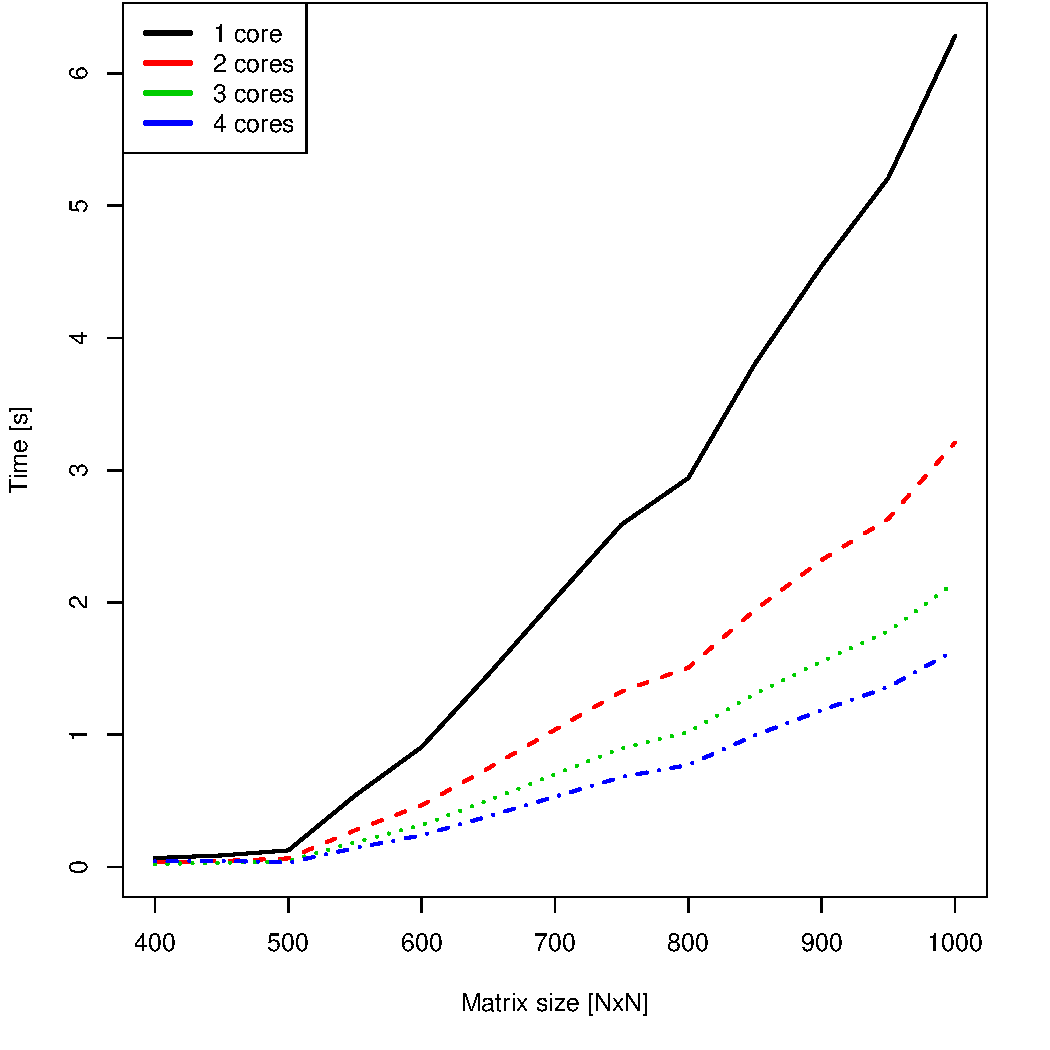
\includegraphics[width=120mm,height = 100mm]{multicore}
\caption{Porównanie czasu wykonywania się algorytmu mnożenia macierzy dla różnej ilości rdzeni (procesor Intel Core I7 3770K).}
\caption*{Źródło: Obliczenia własne}
\label{cores}
\end{figure}

W przypadku obliczeń równoległych istnieje jednak górne ograniczenie określające maksymalny stopień przyspieszania, który można uzyskać używając wielu procesorów. Niech $S(p,n)$ oznacza krotność przyspieszenia algorytmu równoległego (np. $1$ oznacza brak przyspieszenia, $2$ - algorytm równoległy będzie maksymalnie dwa razy szybszy), dla problemu wielkości $n$, przy użyciu $p$ procesorów, a $s$ udział sekwencyjnej części w całym programie, wtedy:

\begin{equation}
S(p,n) \leq \frac{1}{s+(1-s)/p}.
\end{equation}

Powyższy wzór nosi nazwę prawa Amdhala i służy do wyznaczania górnego ograniczenia przyspieszenia jako funkcji $s$ i $p$ przy ustalonym $n$.  Więcej informacji na temat oceny algorytmów równoległych można znaleźć w \cite{Czech2010}. Również w przypadku niektórych algorytmów zastosowanie technik programowania równoległego w ogóle nie jest możliwe - taka sytuacja zachodzi w przypadku, gdy kolejny krok algorytmu zależy bezpośrednio od kroku poprzedniego.

Dodatkowym problemem związanym z zastosowaniem programów równoległych i rozproszonych może okazać się trudność z ich implementacją. Jednak w tym zakresie prowadzone są prace w celu umożliwienia wykorzystania architektury wieloprocesorowej przy jak najmniejszym wysiłku ze strony programisty. W efekcie tych prac powstała w firmie Google platforma MapReduce \cite{mapreduce}, ułatwiająca programowanie klastrów komputerów na wysokim poziomie abstrakcji, to znaczy pewne zadania, takie jak podział problemu na podproblemy, rozkład zadań pomiędzy węzły, synchronizacja wyników, czy podejmowanie działań na wypadek awarii któregoś z węzłów w trakcie obliczeń, są rozwiązane na poziomie tej platformy, przez co ich implementacja nie należy do zadań piszącego algorytm, co z kolei znacznie ułatwia i przyspiesza proces tworzenia potrzebnej aplikacji. 

Istnieje otwarta (oparta na licencji open source) implementacja platformy MapReduce nosząca nazwę Apache Hadoop. Również w przypadku pakietu statystycznego R istnieje i jest rozwijanych kilka pakietów implementujących to podejście, między innymi RHadoop, RHIPE \cite{rhipe}.

Na uwagę zasługuje fakt, iż w ostatnim czasie dostęp do klastrów obliczeniowych, został znacząco ułatwiony, między innymi dzięki możliwości wynajęcia określonej mocy obliczeniowej na pewien okres czasu (na przykład wynajęcie klastra złożonego z 100 węzłów na 10 godzin potrzebnych do wykonania potrzebnej analizy). Rozwiązanie to jest szczególnie interesujące w przypadku małych i średnich przedsiębiorstw, dla których potrzeba wykorzystania dużej mocy obliczeniowej może być sporadyczna, a koszty utrzymania własnej infrastruktury zbyt duże. 


Warto również zwrócić uwagę na rozwijający się dynamicznie sektor obliczeń prowadzonych na GPU\footnote{GPU - (ang. Graphical Procesor Unit) - karta graficzna komputera}. Rysunek \ref{cuda} pokazuje czas wykonywania się algorytmu mnożenia macierzy na karcie graficznej NVidia GT640 z zastosowaniem technologi CUDA.    

\begin{figure}[H]
\centering
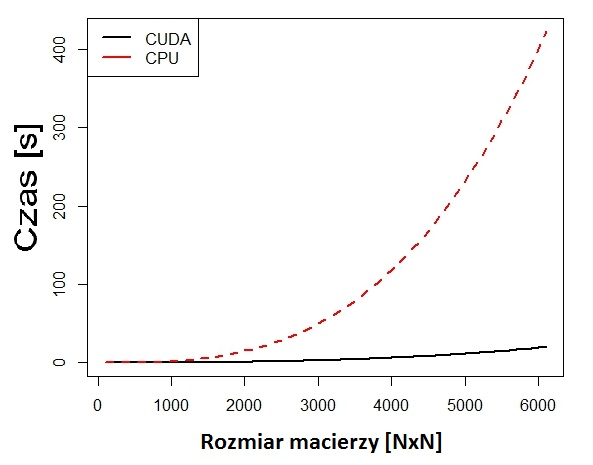
\includegraphics[width=110mm,height = 70mm]{cpuvsgpu}
\caption{Porównanie czasu wykonywania się mnożenia macierzowego dla implementacji na procesorze i karcie graficznej.}
\caption*{Źródło: Obliczenia własne}
\label{cuda}
\end{figure}

Zdaniem autora programowanie kart graficznych w obecnym stadium rozwoju jest zbyt trudne i czasochłonne z perspektywy statystyka czy analityka, gdyż w czasie budowania programu należy mieć na uwadze bardzo niskopoziomowe zagadnienia związane z zarządzaniem pamięcią, przesyłaniem danych z karty graficznej (w większości przypadków pamięć operacyjna nie jest współdzielona pomiędzy procesorem i kartą graficzną), równomiernym obciążeniem procesorów strumieniowych itd. Jednak również w tym zakresie prowadzone są prace nad stworzeniem odpowiednich narzędzi ułatwiających korzystanie z obliczeń na procesorach GPU - przykładem może być dodatek do środowiska MatLab firmy MathWorks\cite{matgpu} jak i pakiety do R - np ,,gputools'' i ,,Rpgu''. 

Należy również zwrócić uwagę, iż w obecnych superkomputerach spora część mocy obliczeniowej pochodzi właśnie z układów GPU. Więcej na temat obliczeń na kartach graficznych można znaleźć w \cite{sanders2011}\cite{kirk2010}.

\subsection{Rozwój technologii a wielkie zbiory danych}

Na zakończenie paragrafu związanego z rozmiarem problemu zostanie krótko omówiony problem zasygnalizowany przez Petera Hubera w \cite{Huber2011}:

\begin{quote}
,,Czy zwiększenie wydajności komputerów zwiększyło moc czy wygodę?''
\end{quote}

Odpowiedź na to pytanie nie mieści się w zakresie tej pracy. Pewne wyobrażenie o problemie może  dać symulacja przygotowana przez autora, porównująca czas wykonywania się naiwnego algorytmu obliczania głębi regresyjnej 2d dla procesorów domowych pochodzących z roku 2008 (Intel Core 2 duo) i roku 2012 (Intel Core I7 3770K). Jej wyniki zaprezentowano na rysunku \ref{i7vs2duo}.

\begin{figure}[H]
\centering
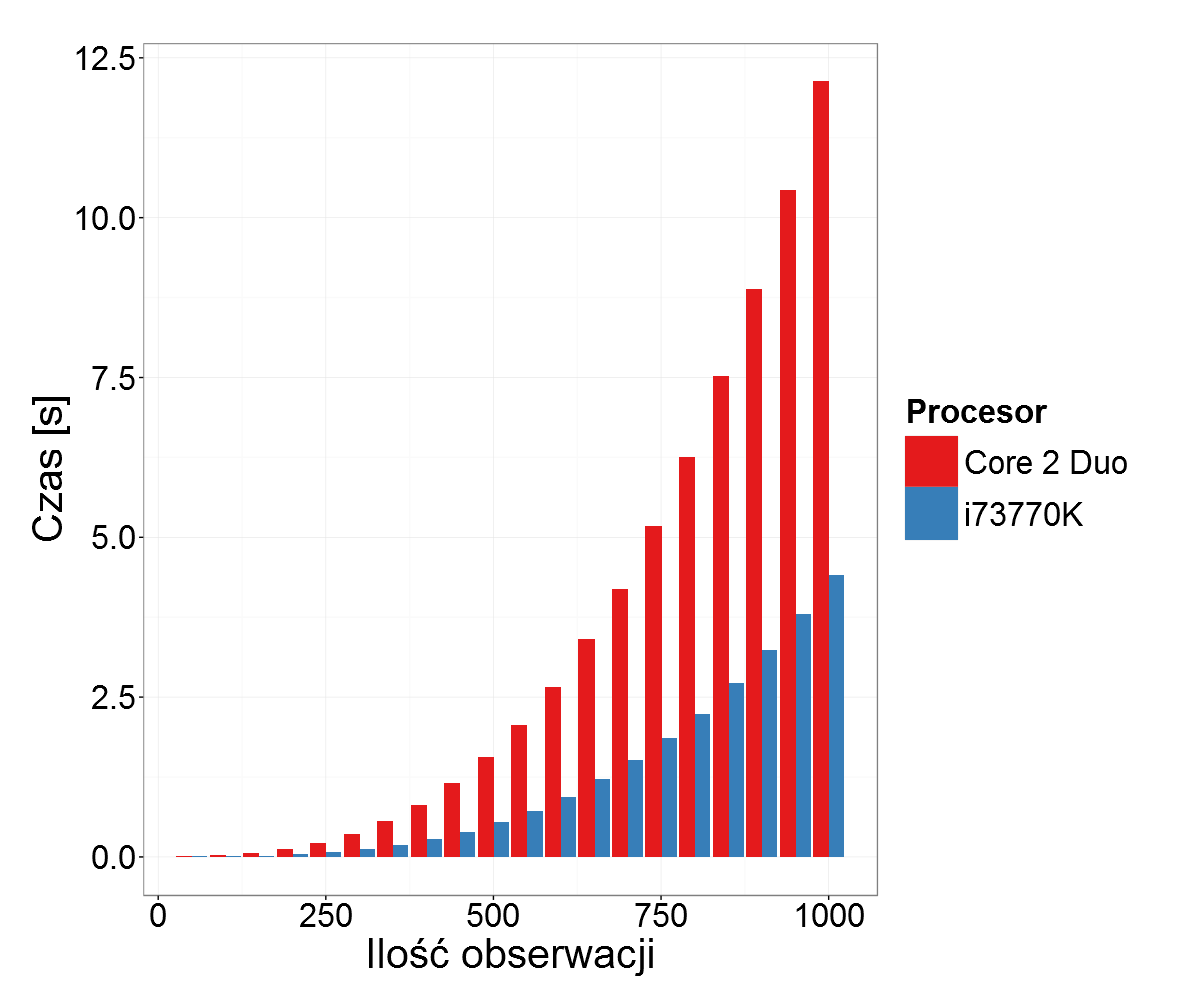
\includegraphics[width=120mm,height = 80mm]{deepregtest}
\caption{Porównanie czasu wykonania naiwnego algorytmu obliczania głębi regresyjnej 2d dla procesorów Intel Core I7 3770K (rok 2012) i Intel Core 2 duo (rok 2008).}
\caption*{Źródło: Obliczenia własne}
\label{i7vs2duo}
\end{figure}

W tym przypadku uzyskano około trzykrotne przyspieszenie. Po upływie 4 lat w tym samym czasie, dla tego algorytmu jest się w stanie rozwiązać problem większy o około 50\%.

\section{Szybkość napływania nowych danych}

Drugą cechą charakteryzującą wielki zbiór danych jest szybkość napływania nowych obserwacji, co jednocześnie wiąże się z tempem w jakim zbiór się powiększa. Najprostszym przykładem zbioru powiększającego się w dynamiczny sposób są dane giełdowe, gdzie ceny transakcyjne i informacje o zmianach na książce zleceń pojawiają się w krótkich interwałach, często wielokrotnie w ciągu sekundy. Problemy i sposoby radzenia sobie w przypadku danych o dużej częstotliwości zostaną szerzej omówione w dalszej części pracy dotyczącej zagadnienia strumieni danych.

\section{Struktura zbioru}

Złożoność struktury zbioru można rozumieć dwojako. Po pierwsze - złożoność pod kątem informacji, których dotyczą dane znajdujące się w zbiorze. Przykładem może być zbiór danych ze spisu powszechnego, w którym znajdują się informacje dotyczące wielu aspektów gospodarki, demografii itd. Po drugie - pod względem sposobu zapisu danych - czy w łatwy sposób można wydobyć interesujące dane? 

Pierwszy przypadek traktowania złożoności struktury zbioru pod kątem ilości informacji w nim zawartych wydaje się być raczej powodem dla którego analizuje się wielkie zbiory danych, niż problemem z którym należy się zmierzyć. W takim przypadku użyte narzędzia i napotkane trudności zależeć będą od informacji, które badacz chce uzyskać na podstawie danego zbioru. Z faktu, iż jest to temat zbyt obszerny autor ogranicza się do przedstawienia problemów związanych z drugim sposobem rozumienia złożoności zbioru jako sposobu jego magazynowania i postaci danych jakie się w nim znajdują.

Trudność związana z magazynowaniem wielkich zbiorów danych nie zależy jedynie od jego fizycznego rozmiaru (rozumianego w kontekście przestrzeni dyskowej), ale również od innych parametrów które chcemy uzyskać, na przykład:
\begin{itemize}
\item zachowanie określonych relacji, bądź hierarchii w danych,
\item wysoka dostępność danych,
\item wysoka przepustowość bazy danych.
\end{itemize}

W przypadku próby zachowania określonych relacji pomiędzy danymi naturalnym rozwiązaniem jest zastosowanie relacyjnego modelu bazy danych. W takim podejściu dostęp do interesujących danych jest w znacznym stopniu ułatwiony, odbywa się to jednak kosztem innych właściwości, takich jak przepustowość i czas dostępu, które w innych zagadnieniach mogą mieć bardziej kluczowe znaczenie. Przykładowo firma  Google opracowała własną, nierelacyjną bazę danych BigTable\cite{bigtable}, która pozwala na analizę 20 petabajtów $2\cdot 10^{16}$ danych dziennie\cite{nosql}. Rozmiar ten w znaczący sposób wykracza poza przedstawioną skalę klasyfikującą zbiór danych według rozmiaru.

\subsection{Wizualizacja wielkiego zbioru danych}

W przypadku klasycznej analizy statystycznej badacz ma dostęp do szerokiego spektrum metod wizualizacji danych, jednak dla wielkich zbiorów danych wizualizacja może być utrudniona. Pierwszym problemem jest sam rozmiar zbioru, przez który interesujące zależności (np. obszary podwyższonej gęstości) mogą być niewidoczne na wykresie.

Na rysunku \ref{bigvis1} została zaprezentowana jedna z możliwych metod pozwalającą lepiej przedstawić na wykresie punktowym zbiór danych o liczebności $10^6$ obserwacji (w przykładzie są to dane wylosowane z dwuwymiarowego rozkładu normalnego). Polega ona na wypełnieniu punktu na wykresie tylko w określonym stopniu tak, by dopiero określona z góry ilość punktów nakładających się na siebie dawała pełne wypełnienie.

\begin{figure}[H]
\centering
 \begin{subfigure}[t]{0.35\textwidth}
  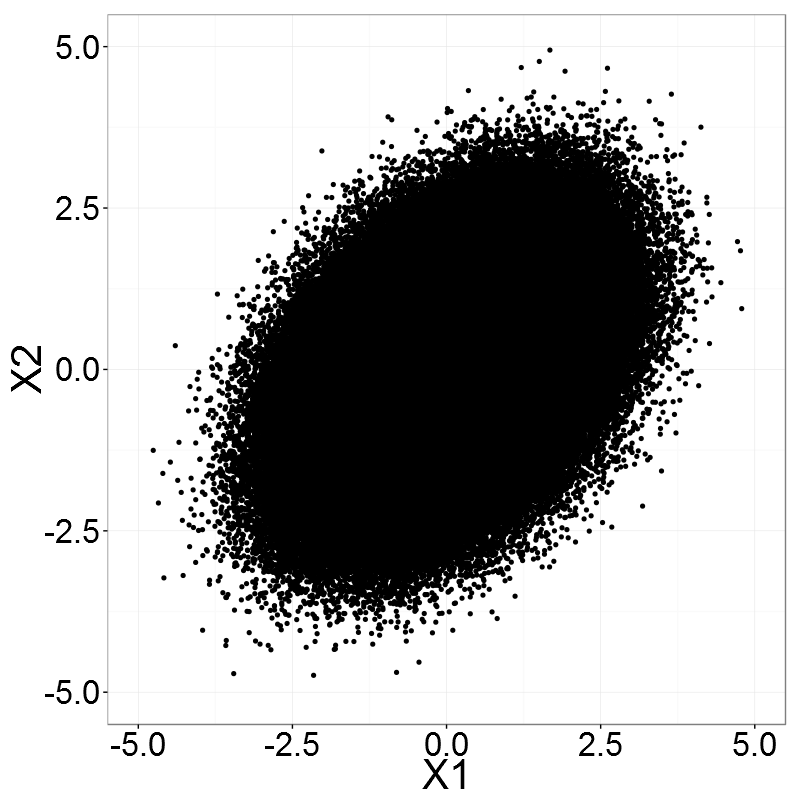
\includegraphics[width=\linewidth]{big1.png}
  \caption{Bez zastosowania wyżej omawianej metody.}
\end{subfigure}
 \begin{subfigure}[t]{0.35\textwidth}
  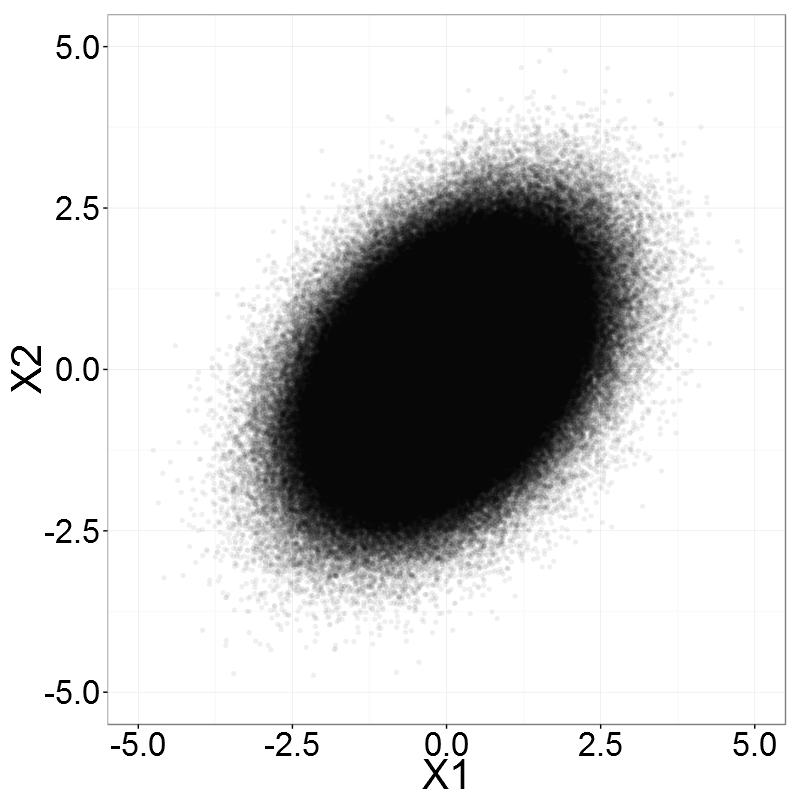
\includegraphics[width=\linewidth]{big2.png}
 \caption{Z zastosowaniem wyżej omówionej metody - obszar o mniejszej gęstości na obrzeżach zbioru jest lepiej widoczny.}
\end{subfigure}
\caption{Prosta wizualizacja zbioru danych zawierającego $10^6$ obserwacji}
\caption*{Źródło: Obliczenia własne - R Project}
\label{bigvis1}
\end{figure}

Kolejnym sposobem (będącym jednocześnie rozwinięciem metody zaprezentowanej powyżej) jest podział przestrzeni na komórki i zliczenie obserwacji należących do poszczególnych komórek i na tej podstawie określenie poziomu wypełnienia punktu na wykresie, będącego reprezentacją pojedynczej komórki. Powyższą metodę zastosowano w pakiecie "bigvis"\cite{bigvis} środowiska R. Rysunek \ref{bigvis2} utworzono przy zastosowaniu tego pakietu.

\begin{figure}[H]
\centering
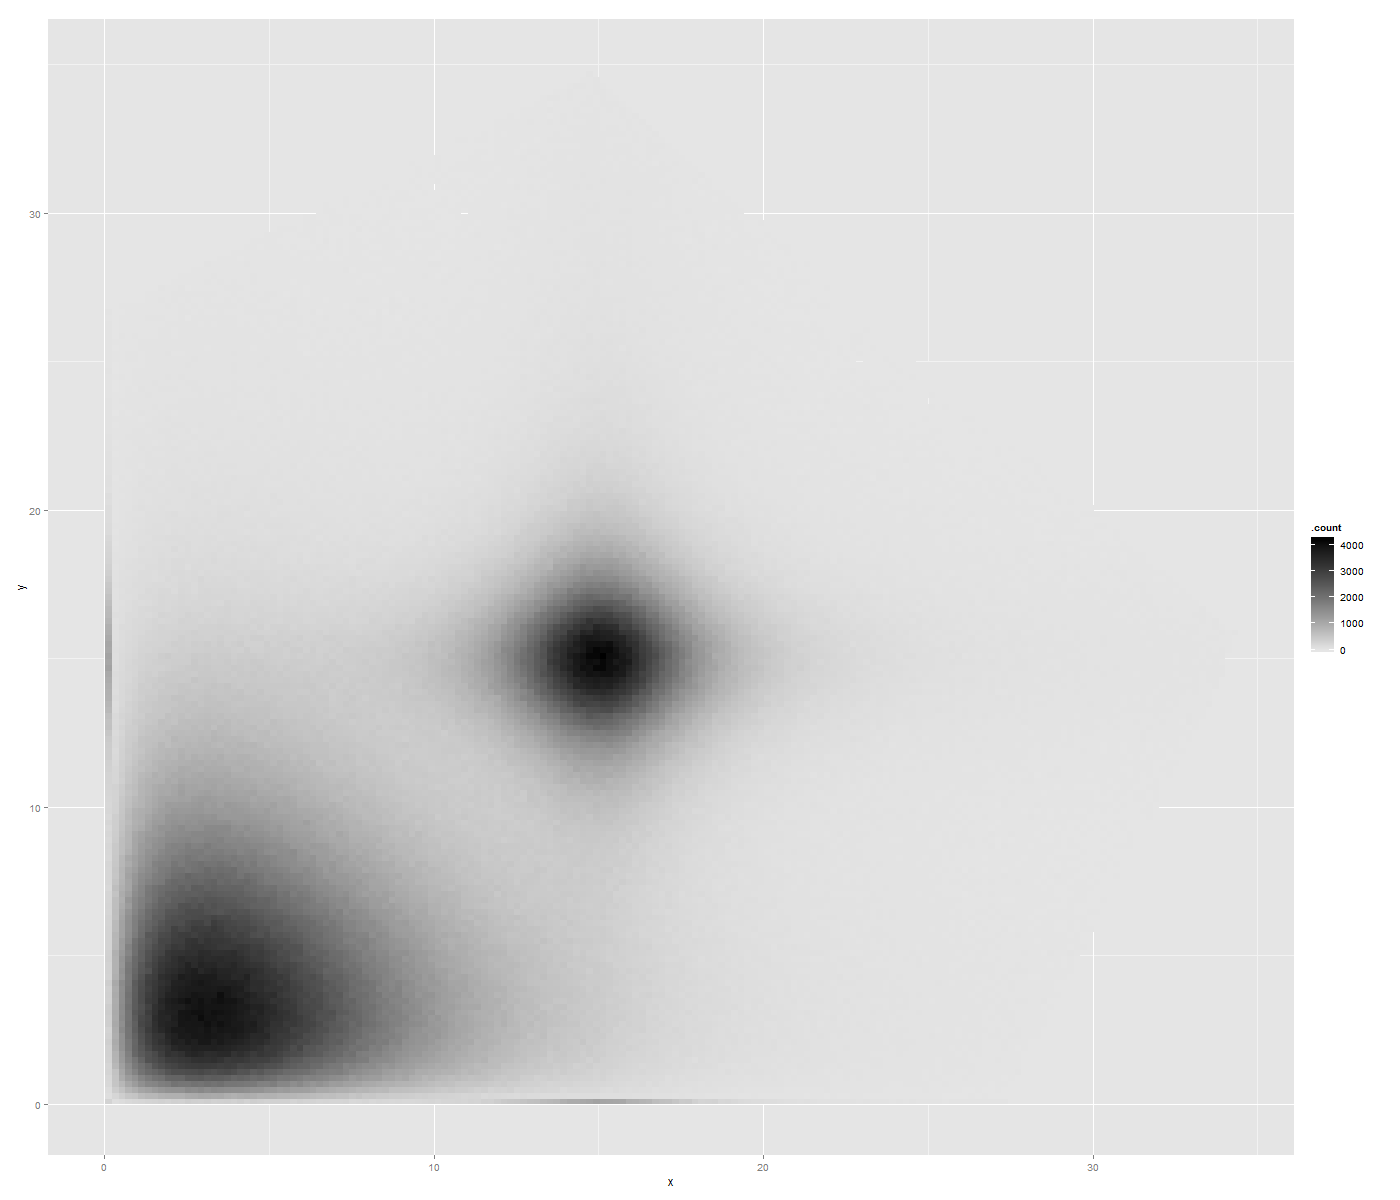
\includegraphics[width=100mm,height = 50mm]{bigvisex}
\caption{Wizualizacja przykładowego zbioru danych zawierającego $10^8$ obserwacji przy użyciu pakietu ,,bigvis'' środowiska R}
\caption*{Źródło: Obliczenia własne - R Project, pakiet bigvis}
\label{bigvis2}
\end{figure}

Więcej na temat wizualizacji wielkich zbiorów danych można znaleźć w: \cite{graphprism} - wizualizacja struktury sieciowej, \cite{sas} - sposoby przedstawiania wielkich zbiorów danych w programie SAS, \cite{bigtext} - prezentacja danych tekstowych.

\chapter{Regresja w zagadnieniu strumieni danych}

Szczególnym zagadnieniem związanym z analizą wielkich zbiorów danych są strumienie danych. Intuicyjnie ,,strumień danych'' można określić jako ciąg obserwacji o nieokreślonej długości. Różnica pomiędzy analizą strumienia, a tradycyjnie rozumianą analizą procesu stochastycznego polega na fakcie, iż w przypadku procesu zakłada się ustalony przedział czasowy [0,T] i na tej podstawie dokonywane są obliczenia. Natomiast w przypadku strumienia danych taki przedział nie jest ustalony, a pojawienie się nowych obserwacji oznacza nową analizę. Analizę strumienia danych można określić jako sekwencję analiz procesu stochastycznego\cite{stream}.

Strumienie danych mają bardzo szerokie zastosowanie praktyczne związane z między innymi z monitorowaniem pracy różnorodnych urządzeń, czy zjawisk (np. w takim przypadku strumieniem mogą wskazania jakiegoś detektora), jak również w przypadku rynków finansowych - analiza danych giełdowych pod kątem wyszukiwania okazji inwestycyjnych. Szczególnie ostatnie zagadnienie związane jest z zainteresowaniami autora i zostanie rozwinięte w dalszej części pracy.

Analiza strumieni danych wiąże się z wieloma wyzwaniami zarówno z punktu widzenia statystyki i informatyki. W pierwszej kolejności zostaną omówione zagadnienia związane z aspektami informatycznymi. 

\subsection{Okno danych - ilość używanych obserwacji do analizy strumienia w określonym momencie czasowym}

Analizę w  przypadku strumieni danych prowadzi się o stale aktualizowaną próbę, najczęściej w oparciu o okno ustalonej długości. 

Niech $\{X_t, t \in \mathbb{N}\} = (X_1,X_2,...)$ oznacza strumień danych, gdzie $X_k$ to k-ta obserwacja pochodząca ze strumienia. Okno $W_{i,n}$ w analizie strumieni danych zdefiniowane jest jako ciąg obserwacji $X_k$ kończących się w $X_i$, o długości $n$: $W_{i,n} = (X_{i-n+1},...,X_i)$.

Rysunek \ref{fig:exwindow} przedstawia przykładowe okno danych. Obserwacje zaznaczone na czerwono, wchodzą w skład okna i na ich podstawie budowany jest model. Kolorem niebieskim przedstawiono obserwacje z przeszłości które nie będą już używane w analizie, szare obserwacje to nieznane w danej chwili wartości strumienia z przyszłości.

\begin{figure}[H]
\centering
\vspace{-10pt}
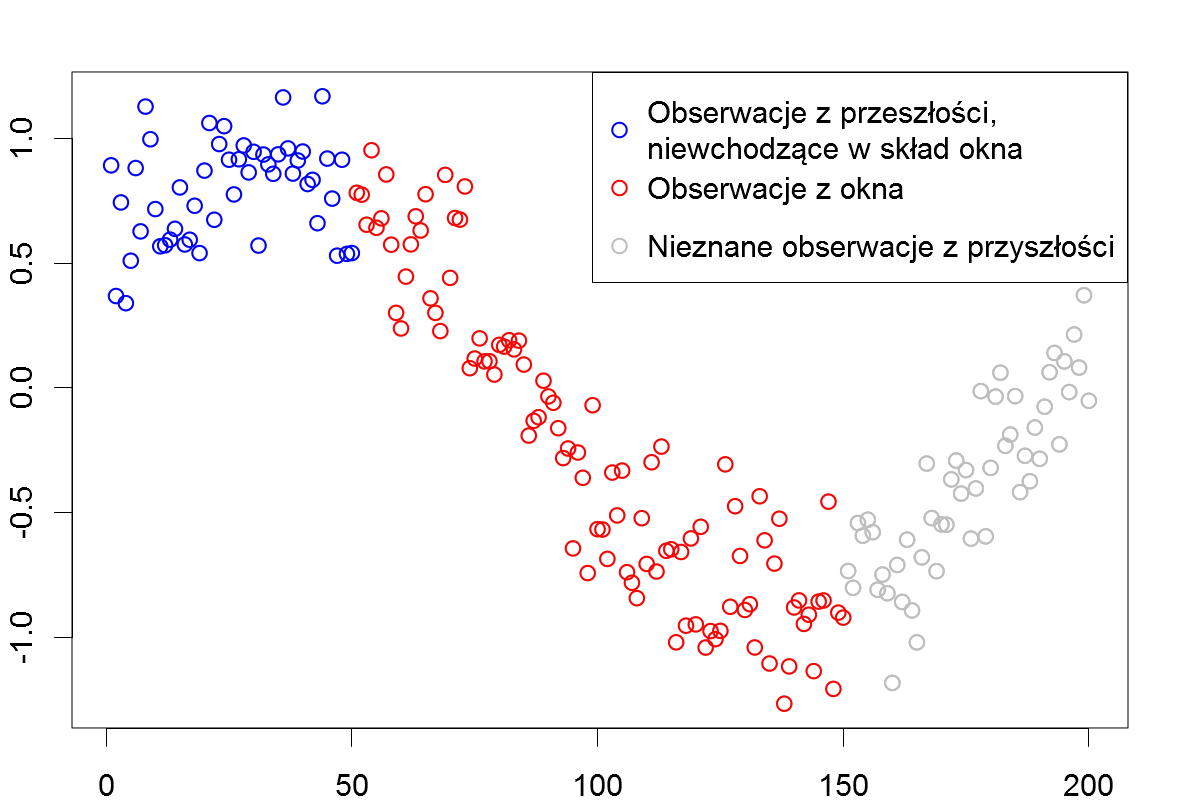
\includegraphics[width=105mm,height = 70mm]{window}
\caption{Przykładowe okno danych}
\caption*{Źródło: Obliczenia własne}
\label{fig:exwindow}
\end{figure}

Długość używanego okna zależy przede wszystkim od badacza i cech procesu które stara się uchwycić. Im dłuższe okno, tym zależności bardziej długoterminowe. Równocześnie można monitorować kilka okien różnej długości, o różnej częstotliwości zbierania danych.

\subsection{Szybkość pojawiania się nowych danych}

Problem związany z szybkością pojawiania się nowych danych został już zasygnalizowany w poprzednim rozdziale, związanym bezpośrednio z wielkimi zbiorami danych - w tej sekcji zostanie on szerzej omówiony.

W przypadku strumieni danych wraz z pojawieniem się nowej informacji używany model powinien zostać zaktualizowany, tak by ująć nową wiedzę. Może jednak zaistnieć sytuacja w której czas potrzebny na przebudowanie modelu znacząco przekracza okres do pojawienia się nowej obserwacji. Najprostszym rozwiązaniem w takiej sytuacji jest zbieranie danych w pakiety określonej wielkości (lub z określonego okresu) i w tej formie przekazywanie ich do modelu. W tym przypadku należy się jednak liczyć z tym, iż decyzje nie są podejmowane w oparciu o najnowszą informację - w wielu zastosowaniach takie podejście jest jednak wystarczające, a nawet pożądane. W przypadku strategii giełdowych w pewnych przypadkach pożądane jest zmniejszenie częstotliwości otrzymywanych danych, tak by zmniejszyć szum związany efektami mikrostruktury rynku\cite{doman}.

Bardzo ciekawym rozwiązaniem z punktu widzenia zarówno praktycznego, jak i algorytmicznego jest użycie, lub zaprojektowanie algorytmu którego złożoność obliczeniowa w momencie jego aktualizacji wynosi $O(1)$ (stała). W tym przypadku na początkowym oknie $W_{i,n}$ można użyć algorytmu, o stosunkowo dużej złożoności obliczeniowej (np. $O(n^3)$), a dla kolejnych okien $W_{i+k,n}$ szybko aktualizować parametry zbudowanego modelu. Natomiast sytuacja w której dla każdego okna należy wykonać tę samą ilość operacji może okazać się nieakceptowalna, gdyż czas potrzebny na ponowną estymację parametrów modelu, może w znaczący sposób przekraczać okres w którym otrzymane wyniki mają sens (np. otrzymanie prognozy pogody na okres 4 najbliższych dni, dopiero po 6 dniach obliczeń, por. \cite{Karbowski2009}).


\section{Metoda najmniejszych kwadratów}

Estymator regresji liniowej metodą najmniejszych kwadratów ma bardzo długą historię, jego pierwsze opisy dokonane przez Carla Fredricha Gaussa  i Adriena-Marie Legendre pochodzą z końca XVIII wieku, jednak ciągle jest bardzo szeroko stosowany.

Modelu w przypadku regresji liniowej ma postać:

\begin{equation}
\mathbf{y} = \mathbf{\theta} \mathbf{X} + \mathbf{\epsilon},
\end{equation}

gdzie, $\mathbf{y}$ to wektor zmiennej objaśnianej, $\mathbf{X}$ jest macierzą zmiennych objaśniających, $\mathbf{\theta}$ to wektor parametrów, natomiast $\mathbf{\epsilon}$ jest to wektor odzwierciedlający wpływ czynników przypadkowych lub nieuwzględnionych w zbiorze zmiennych objaśnianych.

Dana jest próba $\mathbf{Z_N} = \{(\mathbf{x_1},y_1),...,(\mathbf{x_N},y_N)\} \subset \mathbb{R}^{p+1}$, gdzie $\mathbf{x_i} = (x_{1,i},...x_{p,i})$ oznacza i-ty wektor zmiennych objaśniających o liczbie współrzędnych $p$, natomiast $y_i$ i-tą zmienną objaśnianą, $N$ jest to ilość obserwacji w próbie. Estymator MNK zostaje wyznaczony poprzez minimalizację kwadratów reszt \ref{e:mnk}.
\begin{equation}\label{e:mnk}
\mathbf{\hat{\theta}}_{MNK} = argmin(\sum^N_{i=1}(y_i-\mathbf{\theta} \mathbf{x_i})^2).
\end{equation}

Przy założeniach, że zmienne objaśniające są liniowo niezależne, estymator MNK można uzyskać rozwiązując układ równań:

\begin{equation}
\mathbf{\hat{\theta}} = (\mathbf{X}^T\mathbf{X})^{-1}\mathbf{X}^T\mathbf{y}.
\label{equ:est_mnk},
\end{equation}

gdzie $\mathbf{X}^T$ oznacza transpozycję macierzy obserwacji objaśniających, $(\mathbf{X}^T\mathbf{X})^{-1}$ jest macierzą odwrotną do macierzy $\mathbf{X}^T\mathbf{X}$.

Dodatkowo przy założeniach, że:
\begin{itemize}
\item $E(\mathbf{\epsilon})=\mathbf{0}$,
\item $D^2(\mathbf{\epsilon}) = E(\mathbf{\epsilon\epsilon}^T) = \sigma^2\mathbf{I}$ i $\sigma^2<\infty$,
\item $\epsilon_i \sim N(0,\sigma)$,
\end{itemize}
estymator MNK jest klasy BLUE\footnote{ang. 
best linear unbiased estimator - najlepszy nieobciążony liniowy estymator}. $E(\mathbf{\epsilon})$ oznacza wartość oczekiwaną $\mathbf{\epsilon}$, $D^2(\mathbf{\epsilon})$, to macierz kowariancji, $\sigma$ to określona liczba, natomiast $\mathbf{I}$ to macierz jednostkowa.


\subsection{Złożoność obliczeniowa \label{s:zomnk}}

W praktyce z powodów stabilności numerycznej do wyznaczania wektora $\mathbf{\theta}$ nie korzysta się z równania \ref{equ:est_mnk}. Szukany wektor znajduje się poprzez rozwiązanie układu równań normalnych ze względu na $\mathbf{\theta}$:
\begin{equation}
\mathbf{X}^T\mathbf{X\theta} = \mathbf{X}^T\mathbf{y},
\end{equation}
przy pomocy różnych algorytmów dekompozycji macierzy $\mathbf{X}^T\mathbf{X}$. Wykorzystuje się do tego między innymi dekompozycję Choleskiego lub QR.

W przypadku wykorzystania dekompozycji Choleskiego złożoność obliczeniowa algorytmu regresji liniowej wyniesie $O(Np^2+p^3)$, gdzie $N$ to ilość obserwacji, a $p$ to liczba zmiennych objaśniających.

Regresja liniowa posiada również bardzo dobre własności pod kątem użycia w przypadku strumieni danych  i regresji na oknie danych, gdyż pozwala na aktualizację modelu w czasie proporcjonalnym do ilości zmiennych objaśnianych i nie wymaga przetrzymywania danych historycznych.

Poniżej prezentowany jest opis algorytmu szybkiej regresji "IMSR"\cite{imsr}, charakteryzującego się powyższymi własnościami.

Załóżmy, że mamy dane pochodzące z dwóch okresów - okresu do $[0,T]$ i z okresu od $[T+1,T+k]$. Dane z pierwszego okresu dotyczące zmiennych objaśniających znajdują się w macierzy $\mathbf{X_T}$ i reprezentują one wiedzę posiadaną dotychczas, natomiast dane z okresu drugiego znajdują się w macierzy $\mathbf{X_K}$ (reprezentują one napływające dane). Cały zbiór danych składający się z $\mathbf{X_T}$ i $\mathbf{X_K}$ znajduje się w $\mathbf{X}$ (reprezentuje on zbiór danych w momencie jego aktualizacji w chwili $T+k$. Łatwo można pokazać, że:
\begin{equation}
\mathbf{X}'\mathbf{X} = \mathbf{X}_T'\mathbf{X}_T + \mathbf{X}_K'\mathbf{X}_K.
\end{equation}
Podobnie jeżeli $\mathbf{y_T}$ będzie zawierać zmienną objaśnianą z pierwszego okresu, $\mathbf{y_K}$ dane napływające, a $\mathbf{y}$ dane połączone, wtedy:
\begin{equation}
\mathbf{X}^T\mathbf{y} = \mathbf{X}_T^T\mathbf{y_T} + \mathbf{X}_K^T\mathbf{y_K}.
\end{equation}

W przypadku aktualizacji modelu nie trzeba wykonywać w każdym kroku kosztownej obliczeniowo operacji mnożenia macierzy $\mathbf{X}'\mathbf{X}$ - wystarczy obliczyć ją jeden raz, a następnie aktualizować o iloczyn $\mathbf{X}_K^T\mathbf{X}_K$. Podobnie w przypadku iloczynu macierzy $\mathbf{X}^T\mathbf{y}$.

Drugą zaletą tego podejścia jest fakt, iż nie jest konieczne przetrzymywanie wszystkich informacji historycznych.


W przypadku regresji na oknie należy zachować macierze którymi aktualizuje się $\mathbf{X}^T\mathbf{X}$ i $\mathbf{X}^Ty$, by po określonej liczbie kroków odjąć je w celu usunięcia zawartej w nich informacji. Ilość macierzy które musimy aktualnie przechowywać jest równa długości okna.

Złożoność obliczeniowa w takim przypadku wynosi $O(Kp^2+p^3)$, gdzie $K$ oznacza ilość obserwacji przekazanych do aktualizacji modelu, przy czym $K<N$.

\section{Estymator największej głębi regresyjnej i jego własności}

Metoda majwiększej głębi regresyjnej (NGR) cechuje się bardzo dobrymi własnościami pod względem odporności, to jest niewrażliwości na obserwacje odstające, bądź nakładanie się lub mieszanie mechanizmów generujących dane\cite{Wielo}.

Dany jest zbiór obserwacji  $\mathbf{Z_N} = \{(\mathbf{x_1},y_1),...,(\mathbf{x_N},y_N)\} \subset \mathbb{R}^{p+1}$, gdzie $\mathbf{x_i} = (x_{1,i},...x_{p,i})$ oznacza i-ty wektor zmiennych objaśniających o liczbie współrzędnych $p$, natomiast $y_i$ i-tą zmienną objaśnianą. $N$ jest to ilość obserwacji w próbie. Celem jest dopasowanie hiperpłaszczyzny afinicznej w $\mathbb{R}^{p+1}$, która $g((\mathbf{x_i},1)\mathbf{\beta}^T) = \beta_1 x_{i,1}+...+\beta_p x_{i,p}+\beta_{p+1}$, gdzie $ \mathbf{\beta} = (\beta_1,...,\beta_{p+1})$

By zdefiniować estymator NGR należy wpierw wprowadzić pojęcie niedopasowania:

\begin{deff}\label{defreg}

Wektor $ \mathbf{\beta} = (\beta_1,...,\beta_{p+1}) \in \mathbb{R}^{p+1}$ nazwiemy niedopasowaniem do $\mathbf{Z_n}$ jeżeli istnieje hiperpłaszczyzna afiniczna $V$ w przestrzeni $X$, taka, że żadne $\mathbf{x_i}$ nie należy do $V$ i reszta $r_i(\mathbf{\beta}) = y_i - g((\mathbf{x_i},1)\mathbf{\beta}^T > 0$ dla wszystkich $x_i$ leżących w jednej z jej otwartych półprzestrzeni, oraz $r_i(\beta) = y_i - g((x_i,1)\beta^T < 0$ dla wszystkich $x_i$ w drugiej otwartej półprzestrzeni.
\end{deff}

\begin{deff}
Głębia regresyjna $rdepth(\mathbf{\beta,Z_n})$ dopasowania $ \mathbf{\beta} = (\beta_1,...,\beta_{p+1}) \in \mathbb{R}^p$ względem zbioru danych $\mathbf{Z_n} \subset \mathbb{R}^{p+1} $ jest najmniejszą liczbą obserwacji, które należy usunąć aby sprawić by wektor $\mathbf{\beta}$ był niedopasowaniem w sensie definicji \ref{defreg}.
\end{deff}


Jako estymator największej głębi regresyjnej definiuje się $\mathbf{\beta}$ takie, że:
\begin{equation}
T^*_r(\mathbf{Z_n}) = max\{rdepth(\mathbf{\beta},\mathbf{Z_n})\}.
\end{equation}


\subsection{Punkt załamania próby skończonej}

Jako punkt załamania próby skończonej definiuje się frakcję obserwacji która sprawia, że estymator staje się bezużyteczny, na przykład jego obciążenie jest zbyt duże.

Punkt załamania próby skończonej (BP - break point) dla estymatora NGR, przy założeniu, że $argmax rdepth(\mathbf{\beta,Z_n}) \geq \frac{n}{p+1}$ i $x_i$ są w ogólnej pozycji\footnote{Zbiór punktów znajduje się z ogólnej pozycji, gdy nie zachodzi w nim przypadek by co najmniej trzy punkty leżały na jednej prostej.} wynosi $\frac{1}{p+1}$ w przypadku gdy dane są osobliwe w jakiś sposób. Można pokazać, że gdy dane pochodzą z założonego modelu wartość BP zbiega z prawdopodobieństwem 1 do wartości $\frac{1}{3}$.

Warto nadmienić, że BP dla estymatora LAD \footnote{ang. Least Absolute Deviations - metoda najmniejszych odchyleń absolutnych.}, uznawanego pierwotnie za metodę odporną, będącego pewną alternatywą dla NGR wynosi 0 \cite{lad}. Estymator ten chroni przed odstawaniem w zakresie zmiennej objaśnianej, jednak nie chroni przed odstawaniem w zakresie zmiennej objaśniającej\footnote{ang. leverage points}. Na wykresach \ref{lad1} i \ref{lad2} zaprezentowano porównanie dla oszacowań MNK, LAD i NGR w przypadku występowania obserwacji odstających.

\begin{figure}[H]

\begin{subfigure}[t]{0.45\textwidth}
  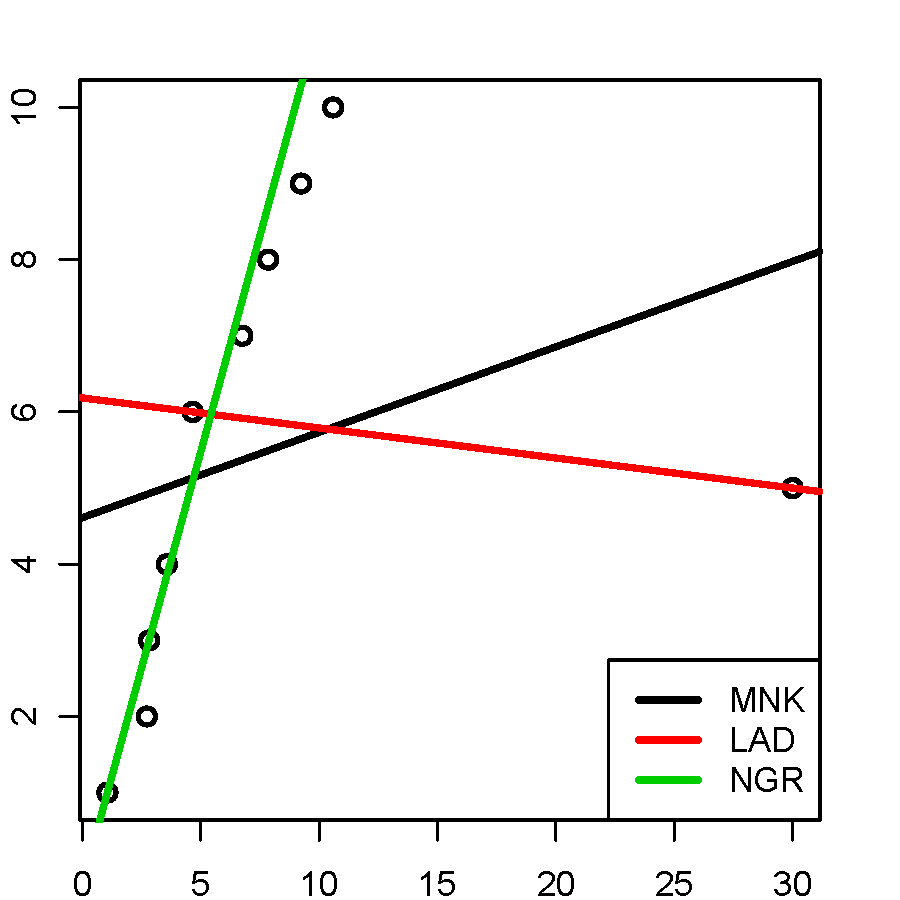
\includegraphics[width=\linewidth]{ladout}
	\caption{Obserwacja odstająca ze względu na zmienną objaśniającą.}
	\label{lad1}  
  
\end{subfigure}
\begin{subfigure}[t]{0.45\textwidth}
  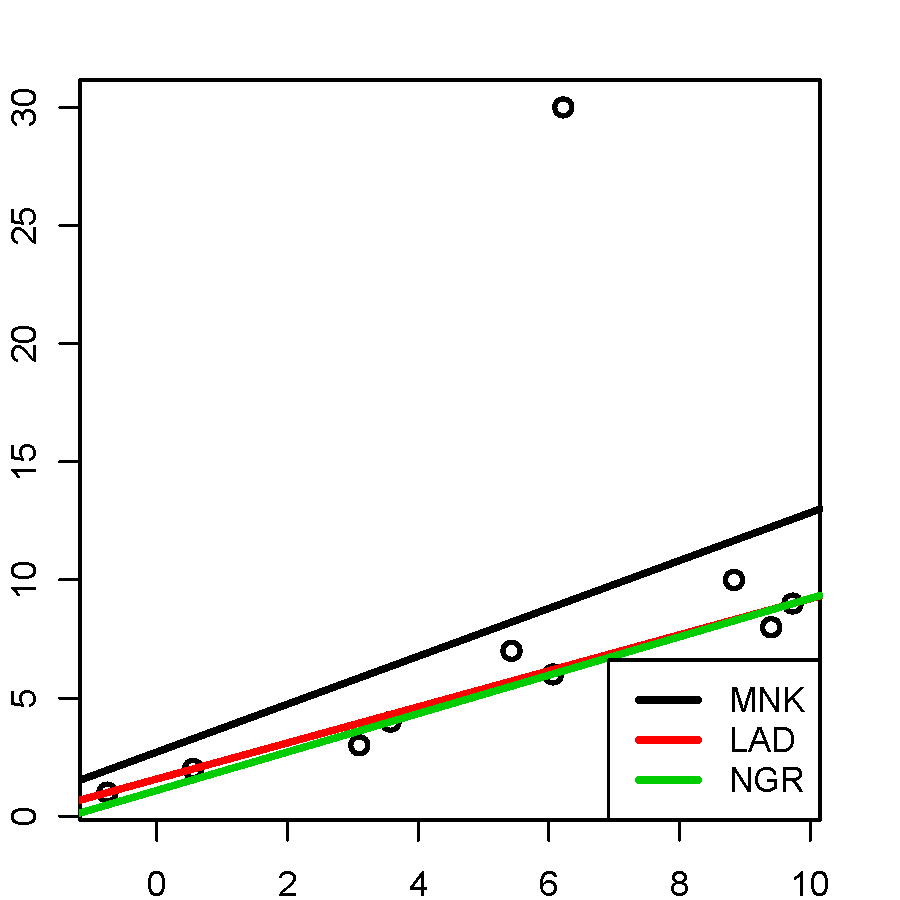
\includegraphics[width=\linewidth]{ladouty}
  \caption{Obserwacja odstająca ze względu na zmienną objaśnianą.}
  \label{lad2}
\end{subfigure}
\caption{Oszacowanie MNK, NGR i LAD w przypadku występowania obserwacji odstających}
\caption*{Źródło: Obliczenia własne - R Project}
\label{fig:lad}
\end{figure}

W obu przypadkach estymator MNK ,,załamuje się'', jego oszacowanie zależy w znacznym stopniu od obserwacji odstającej, natomiast LAD jak zostało wspomniane wyżej jest odporny na obserwację odstającą w zmiennej objaśnianej. W drugim przypadku jego oszacowanie jest zaburzone. Natomiast estymator NGR jest odporny na oba przypadki odstawania.

\subsection{Złożoność obliczeniowa metody największej głębi regresyjnej}

W przypadku dwuwymiarowym złożoność obliczeniowa najlepszego algorytmu wyznaczania dopasowania metodą NGR wynosi $O(n\log n)$\cite{DRM}, w przypadku wyższych wymiarów wyznaczenie dokładnego dopasowania wymaga $O(n^{2p-1}\log n)$ operacji, gdzie $p$ to ilość wymiarów. Taka złożoność obliczeniowa w zasadzie dyskwalifikuje algorytm w przypadku większych zbiorów danych - dla przykładowego zbioru danych mającego $10^4$ obserwacji w 5 wymiarach, oszacowanie parametrów modelu regresji liniowej metodą NGR wymaga wykonania aż $10^{36}$ operacji, co przekracza możliwości obliczeniowe znanych komputerów.

Przy pomocy algorytmu przybliżonego MEEDSWEEP\cite{DRM} oszacowanie NGR można uzyskać w czasie $O(p^2N+hpN+pn \log N)$, gdzie $h$ oznacza liczbę iteracji algorytmu. Złożoność algorytmu MEEDSWEEP nie odbiega w znaczącym stopniu od złożoności algorytmu MNK.

W symulacjach przedstawionych w dalszej części pracy wykorzystano implementację algorytmu największej głębi regresyjnej, pochodzącą z pakietu ,,depthproc'' środowiska R\cite{depthproc}.

\section{Regresja K-najbliższych sąsiadów}

Estymator regresji K-najbliższych sąsiadów (KNN\footnote{ang. K-nearest neighbors - K-najbliższych sąsiadów}) \cite{Hardle1990} jest metodą nieparametryczną, to znaczy, że nie czyni się założeń odnośnie modelu generującego dane. Jego główną zaletą jest prostota konstrukcji i niska złożoność obliczeniowa.

Dana jest próba $\mathbf{Z_N} = \{(\mathbf{x_1},y_1),...,(\mathbf{x_N},y_N)\} \subset \mathbb{R}^{p+1}$, gdzie $\mathbf{x_i} = (x_{1,i},...x_{p,i})$ oznacza i-ty wektor zmiennych objaśniających o liczbie współrzędnych $p$, natomiast $y_i$ i-tą zmienną objaśnianą, $N$ jest to ilość obserwacji w próbie.

Prognozę wartości zmiennej objaśnianej $\mathbf{y_j}$ metodą KNN na podstawie wektora zmiennych objaśniających $\mathbf{x_j}$ wyznacza się jako:

\begin{equation}
\hat{\mathbf{y_j}} = \frac{\sum_{i=1}^N y_i J(\mathbf{x_i},\mathbf{x_j})}{K},
\end{equation}
gdzie:
\begin{equation}
J(\mathbf{x_i,x_j}) = \begin{cases} 1 \text{, gdy $\mathbf{x_i}$ jest jednym z K najbliższych sąsiadów $\mathbf{x_j}$}\\0 \text{, w przeciwnym przypadku} \end{cases},
\end{equation}
natomiast $\mathbf{x_i}$ jest jednym z K najbliższych sąsiadów $\mathbf{x_j}$, w przypadku gdy odległość $d(\mathbf{x_i,x_j})$ należy do K najmniejszych odległości pomiędzy obserwacjami ze zbioru $\mathbf{Z_n}$, a $\mathbf{x_j}$.  Najczęściej wykorzystywane odległości to odległość Euklidesa lub Mahalanobisa, jednak do znalezienia najbliższych sąsiadów można używać koncepcji głębi danych.

W przypadku zastosowania odległości Euklidesa złożoność obliczeniowa regresji KNN wynosi $O(KNp)$, gdzie $K$ to liczba sąsiadów, $N$ to ilość obserwacji w zbiorze $\mathbf{Z_N}$, natomiast $p$, to ilość zmiennych objaśniających.

Regresja KNN nie jest metodą odporną, jednak w przypadku odstawania pod względem zmiennej objaśniającej może radzić sobie lepiej niż regresja MNK (rys. \ref{starsCYG}).

\begin{figure}
\centering
\vspace{-40pt}
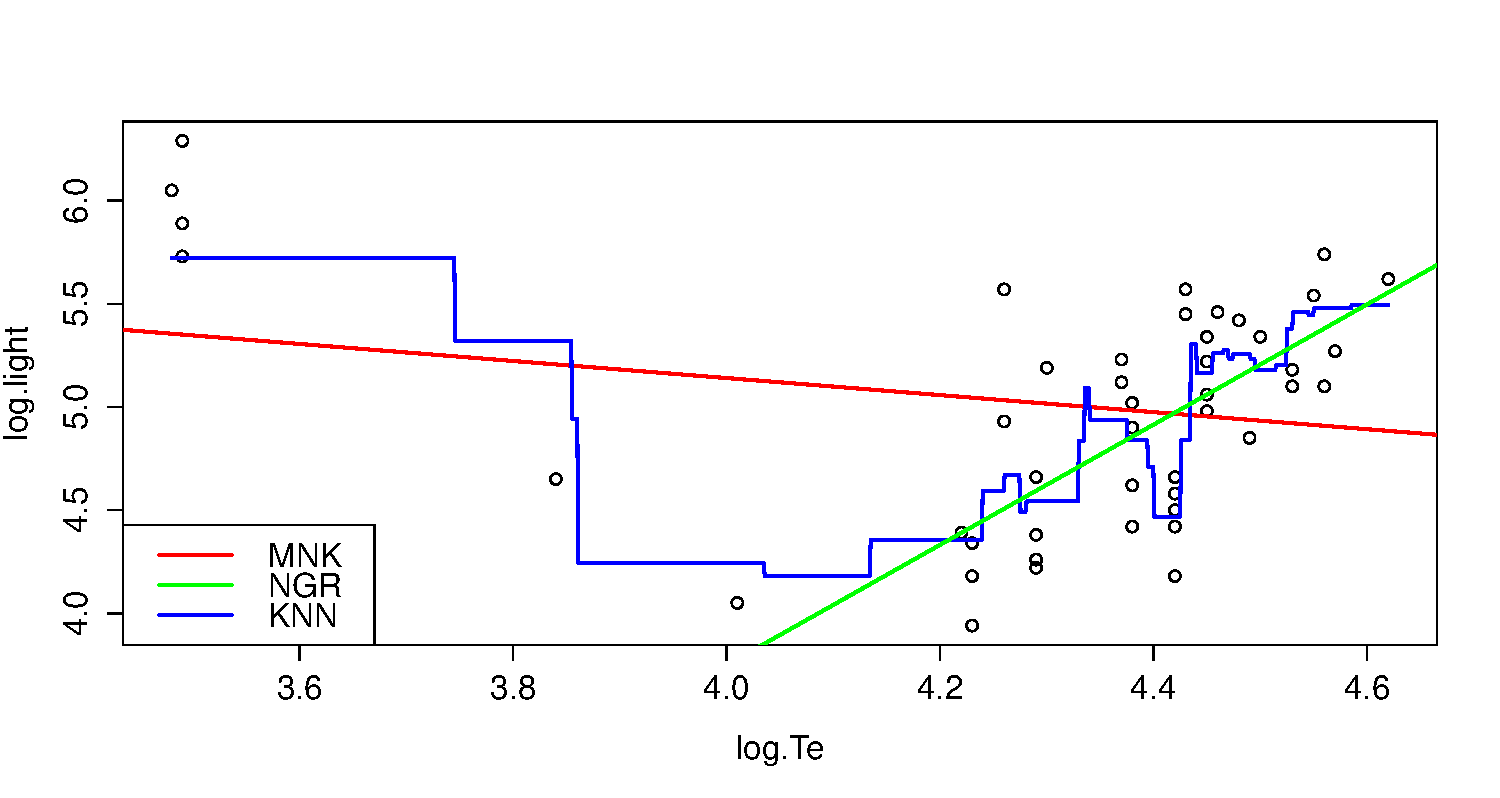
\includegraphics[width=140mm,height = 110mm]{knnplot}
\caption{Oszacowanie regresji KNN, MNK i DRM dla zbioru starsCYG z pakietu robustbase, w przypadku KNN użyto 5 najbliższych sąsiadów.}
\caption*{Źródło: Obliczenia własne - R Project, pakiet robustbase \cite{robustbase}}
\label{starsCYG}
\end{figure}

Również dla zbiorów danych o skomplikowanej strukturze (np. w przypadku zależności nieliniowych) regresja KNN da lepsze wyniki niż metody liniowe (rys. \ref{sinuscosinus}).

\begin{figure}
\centering
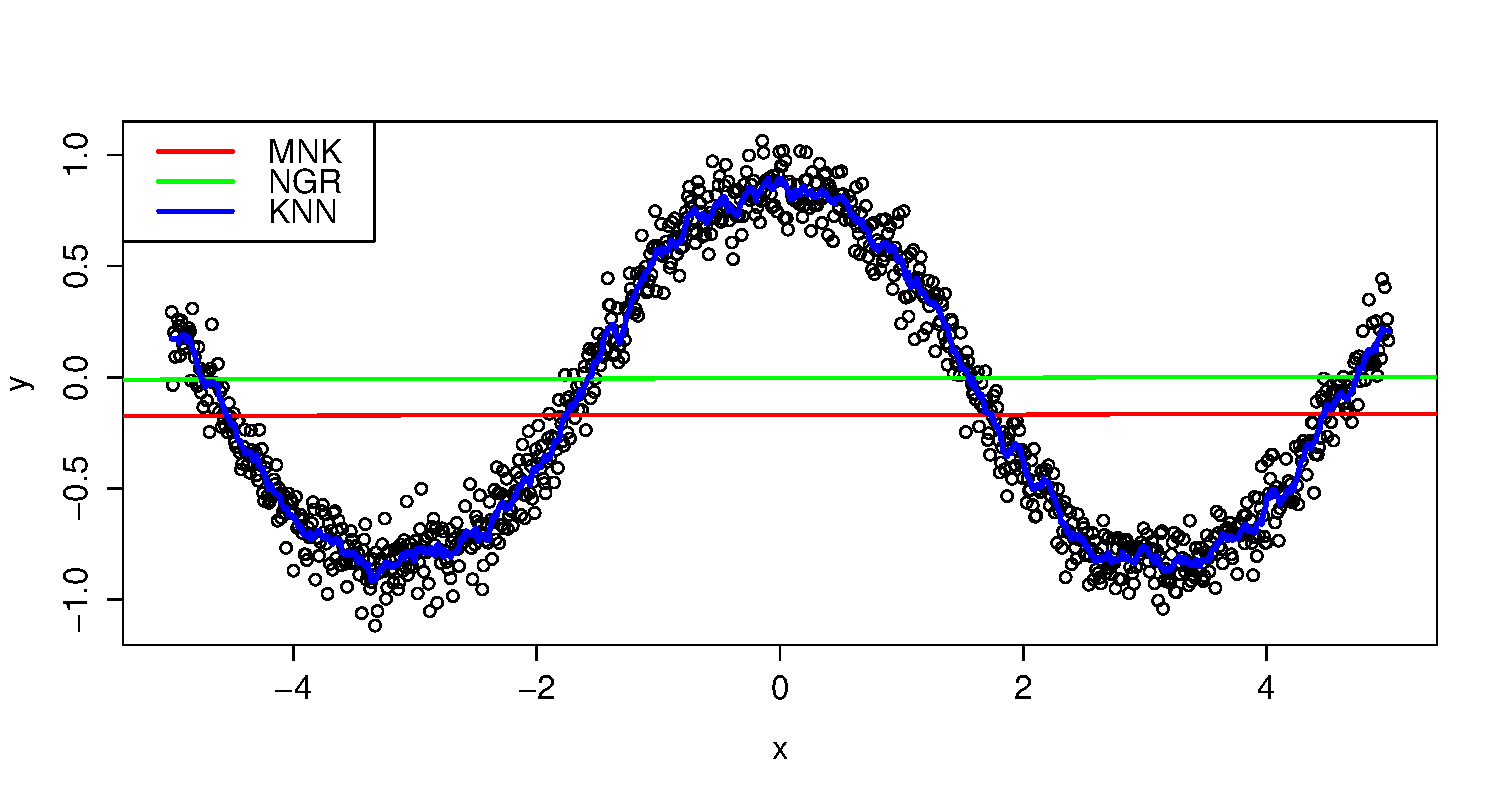
\includegraphics[width=120mm,height = 80mm]{sinknn}
\caption{Oszacowanie regresji KNN, MNK i DRM dla zbioru danych o zależności $y = sin(cos(x))+\epsilon$, $\epsilon \sim N(0,0.1)$.}
\caption*{Źródło: Obliczenia własne - R Project}
\label{sinuscosinus}
\end{figure}

Szerszy opis metod i zastosowań regresji nieparametrycznych można znaleźć w pracy\cite{Ania}.


\section{\label{s:lab}Odporność procedury statystycznej w przypadku ruchomego okna}

Należy jednak zauważyć, że w pewnych zastosowaniach odporność procedury statystycznej może nie zawsze być cechą pożądaną. W dalszej części przedstawiono krótkie rozumowanie przedstawiające kiedy taka sytuacja może zaistnieć.

Przypuśćmy, iż monitorujemy pewien strumień danych $\{y_t, t \in \mathbb{N}\}$, a celem jest przewidywanie następnej obserwacji w oparciu o ruchome okno $W_{t,20}$. Prognoza następnej wartości wyznaczana jest na podstawie modelu:
\begin{equation}\label{e:model}
y_t = \alpha + \beta \cdot t,
\end{equation}
gdzie $t$ oznacza moment w czasie. Parametry $\alpha$ i $\beta$ estymowane są przy użyciu metod MNK i NGR na podstawie obserwacji pochodzących z okna $W_{t,20}$. Na poniższych rysunkach (rys. \ref{fig:start}, rys. \ref{fig:middle}) czerwonym kolorem zaznaczono obserwacje, które w danej chwili używane są do estymacji. W pewnej ustalonej chwili T = 41 następuje zmiana procesu generującego dane - pierwotnie pochodziły one z:
\begin{equation}
y_t = 2 + t + \epsilon.
\end{equation}
Po zmianie:
\begin{equation}
y_t = 1 + 0.5\cdot t + \epsilon,
\end{equation}
gdzie $\epsilon \sim N(0,0.1)$.

Na wykresie \ref{fig:start} przedstawione są oszacowania regresji metodą najmniejszych kwadratów (regresja nieodporna) i największej głębi regresyjnej (metoda odporna) tuż przed zmianą reżimu w oparciu o okno $W_{40,20}$. W tym przypadku wskazania obu estymatorów są bardzo zbliżone.

\begin{figure}[h]
\vspace{-15pt}
\centering
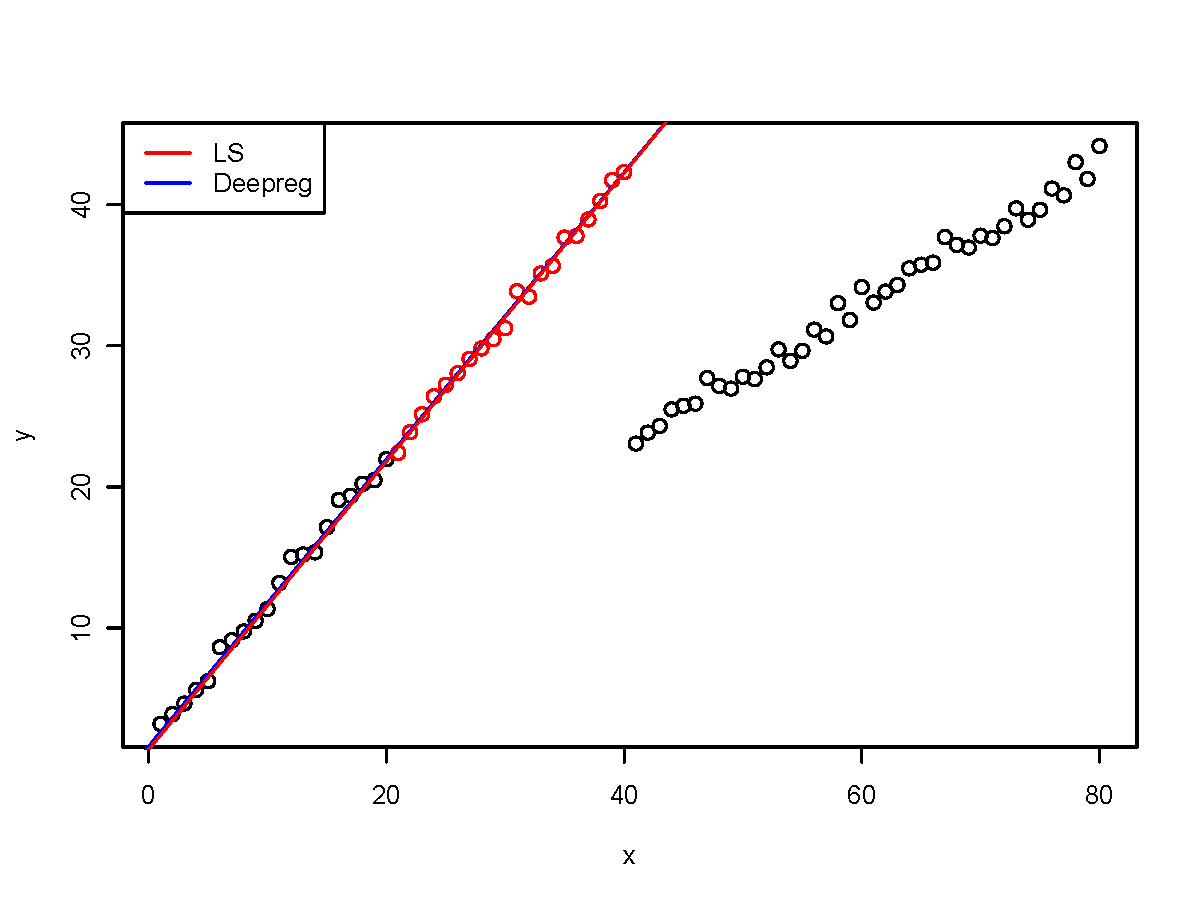
\includegraphics[width=90mm,height = 60mm]{start}
\caption{Oszacowanie przed zmianą reżimu}
\caption*{Źródło: Obliczenia własne - R Project}
\label{fig:start}
\end{figure}

Wykres \ref{fig:middle} przedstawia oszacowanie już po zmianie reżimu w którym 5 obserwacji (25\% okna) pochodzi z drugiego reżimu. 

\begin{figure}[H]
\centering
\vspace{-10pt}
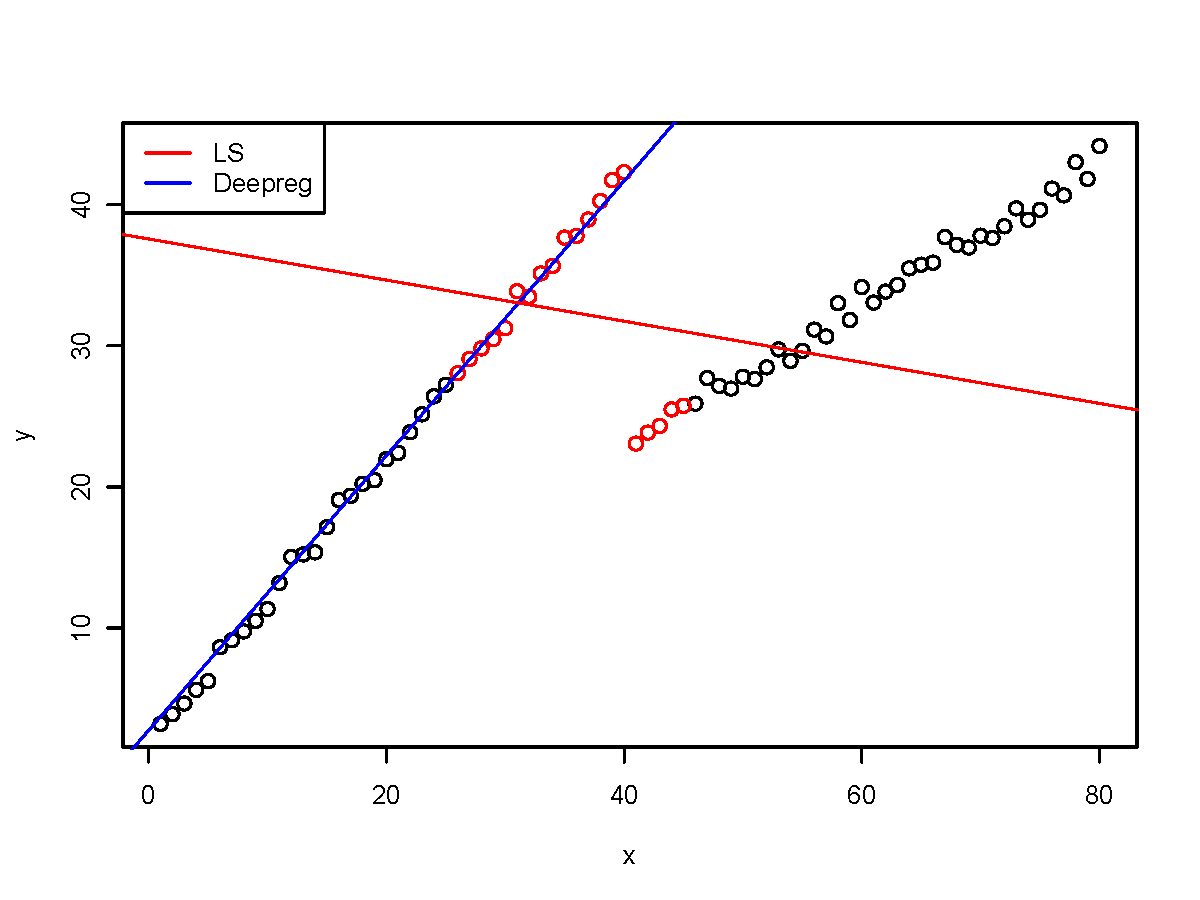
\includegraphics[width=100mm,height = 60mm]{middle}
\caption{Oszacowanie po zmianie reżimu, część obserwacji (15) pochodzi ze starego modelu generującego dane, 5 - z nowego.}
\caption*{Źródło: Obliczenia własne - R Project}
\label{fig:middle}\vspace{-10pt}
\end{figure}

MNK przesunęła się w stronę nowych obserwacji, natomiast NGR nadal wskazuje na poprzedni model. Na rysunku \ref{fig:epsilon} przedstawiono odchylenia predykcji następnej obserwacji od faktycznie zaobserwowanej wartości, wyznaczane jako:
\begin{equation}\label{e:eps}
\hat{\epsilon}_{t} = y_{t} - \hat{E}(y_{t}|W_{t-1,k}),
\end{equation}
gdzie $\hat{\epsilon}_{t}$ to ocena odchylenia w chwili $t$, $y_{t}$ -  wartość strumienia w chwili $t$, $\hat{E}(y_{t}|W_{t-1,k})$ to prognoza warunkowej wartości oczekiwanej, wyznaczona na podstawie modelu \ref{e:model} estymowanego w oparciu o okno $W_{t-1,k}$, $k$ to ilość obserwacji w oknie, w tym przypadku 20.

Należy zwrócić uwagę iż w przypadku MNK wraz z pojawianiem się nowych obserwacji błąd się zmniejsza, natomiast w przypadku NGR w pewnym momencie następuje gwałtowna zmiana z dużej wartości odchylenia od rzeczywistej wartości, do bliskiej zeru.

\begin{figure}[H]
\centering
\vspace{-10pt}
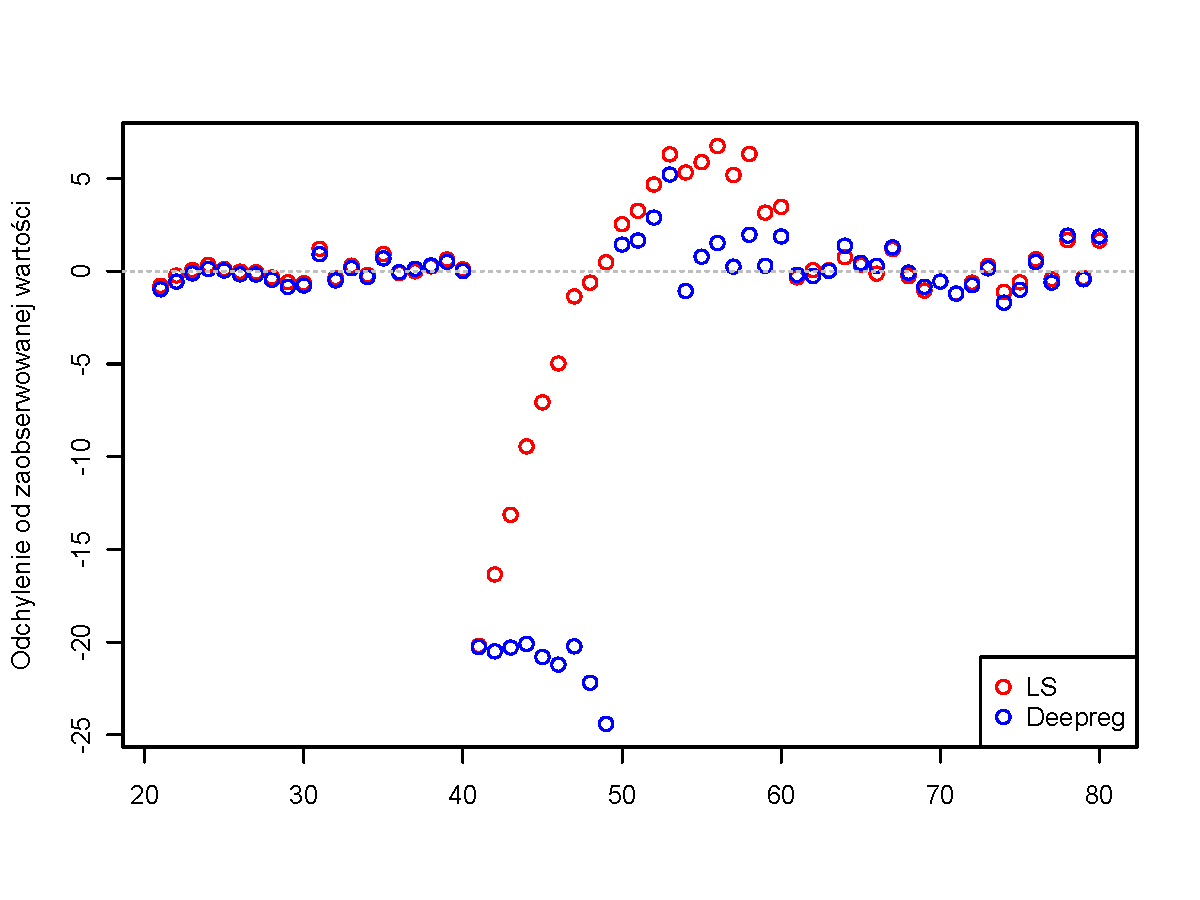
\includegraphics[width=100mm,height = 60mm]{strepsilon}
\caption{Różnica pomiędzy przewidywaną obserwacją a zaobserwowaną w przypadku zmiany reżimu.}
\caption*{Źródło: Obliczenia własne - R Project}
\label{fig:epsilon}
\vspace{-10pt}
\end{figure}

Na kolejnych dwóch wykresach (rys. \ref{fig:intercept} i rys. \ref{fig:beta}) zaprezentowano oszacowania parametrów modelu na kolejnych oknach. Należy zwrócić uwagę, iż w również w przypadku NGR w pewnym momencie obliczone parametry znacznie odbiegały od obu modeli. 

\begin{figure}[H]
\vspace{-10pt}
\begin{subfigure}[t]{0.35\textwidth}
  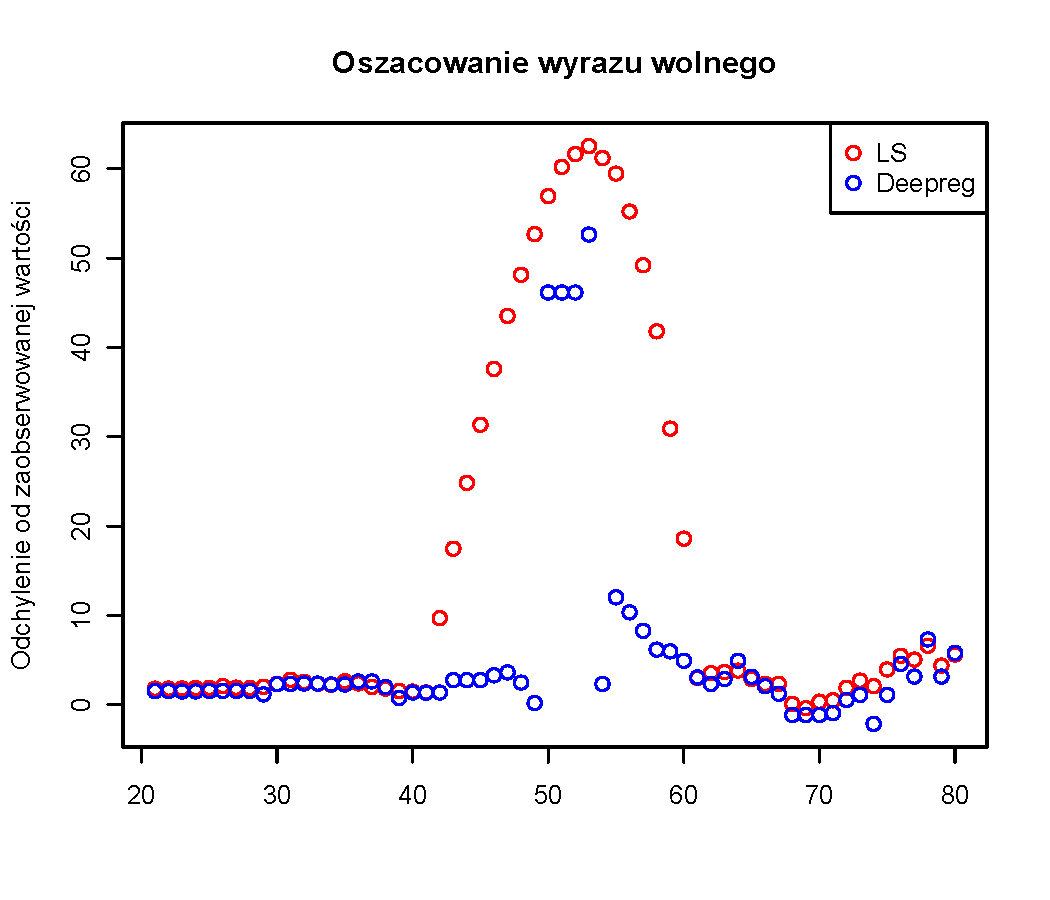
\includegraphics[width=\linewidth]{intercept}
  \caption{Oszacowanie wyrazu wolnego}
  \label{fig:intercept}
\end{subfigure}
\begin{subfigure}[t]{0.35\textwidth}
  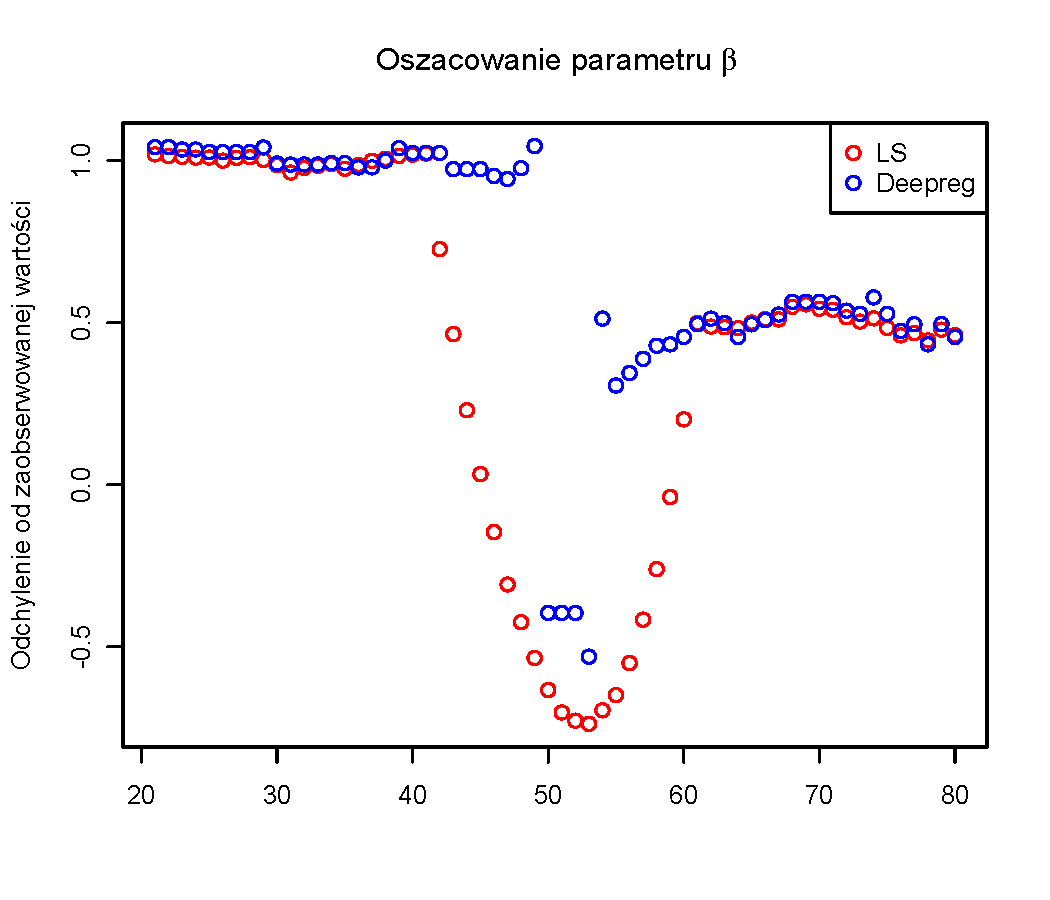
\includegraphics[width=\linewidth]{beta}
  \caption{Oszacowanie parametru nachylenia}
  \label{fig:beta}
\end{subfigure}
\caption{Oszacowania parametrów MNK i NGR w przypadku zmiany reżimu}
\caption*{Źródło: Obliczenia własne - R Project}
\vspace{-10pt}
\end{figure}

Powyższy przykład wskazuje, że w pewnych sytuacjach brak odporności procedury może być zaletą - błędy związane z przewidywaniem następnej obserwacji były mniejsze w przypadku MNK. 

Dla zachowania kompletności rozumowania należy również przedstawić zachowanie się obydwu procedur w przypadku gdy cecha odporności jest pożądana, to jest gdy pojawiają się obserwacje odstające.

Na rysunku \ref{fig:middle2} przedstawiono krzywą regresji w momencie pojawienia się obserwacji odstającej (na wykresie zaznaczona brązowym kolorem, tak jak powyżej punkty użyte do estymacji są czerwone):

\begin{figure}[H]
\centering
\vspace{-10pt}
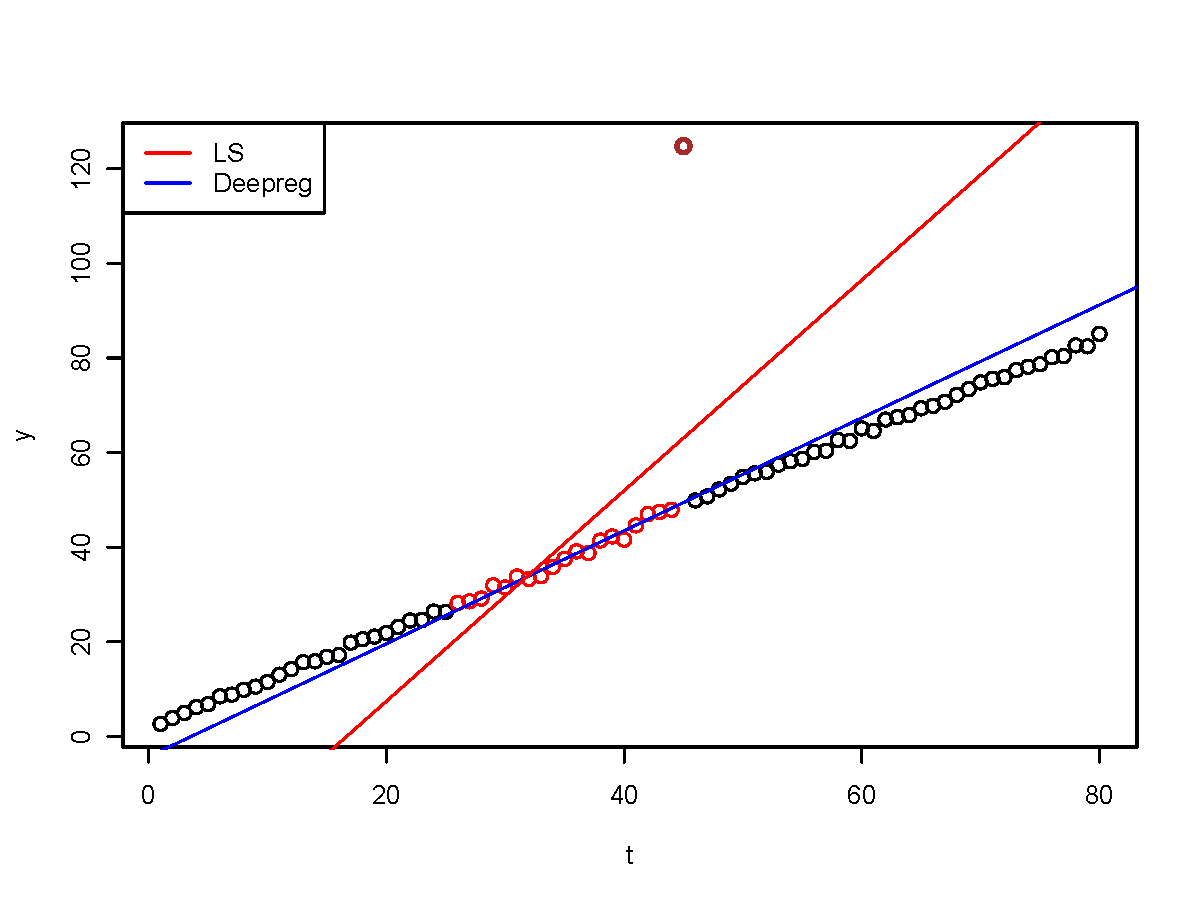
\includegraphics[width=100mm,height = 60mm]{middle2}
\caption{Krzywa regresji w przypadku pojawienia się obserwacji odstającej.}
\caption*{Źródło: Obliczenia własne - R Project}
\label{fig:middle2}\vspace{-10pt}
\end{figure}

Wykresy \ref{fig:interceptout} i \ref{fig:betaout} prezentują oszacowania parametrów modelu dla kolejnych okien w przypadku występowania obserwacji odstającej, liczone według wzoru \ref{e:eps}. Oszacowania parametrów MNK przez okres w którym obserwacja odstająca znajduje się w oknie używanym do estymacji modelu, znacznie odbiegają od procesu generującego dane. Natomiast w przypadku NGR nie występuje żadna istotna zmiana.

\begin{figure}[H]
\centering
\begin{subfigure}[t]{0.40\textwidth}
  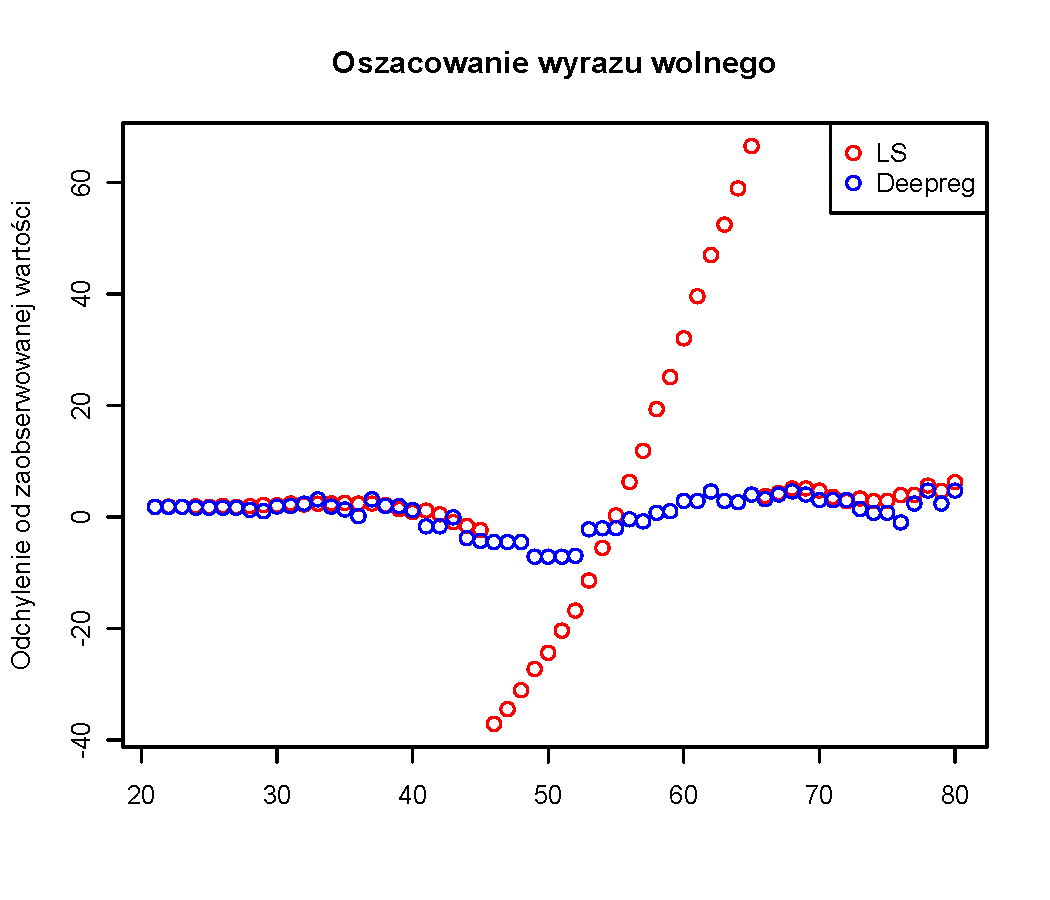
\includegraphics[width=\linewidth]{interceptout}
  \caption{Oszacowanie wyrazu wolnego}
  \label{fig:interceptout}
\end{subfigure}
\begin{subfigure}[t]{0.40\textwidth}
  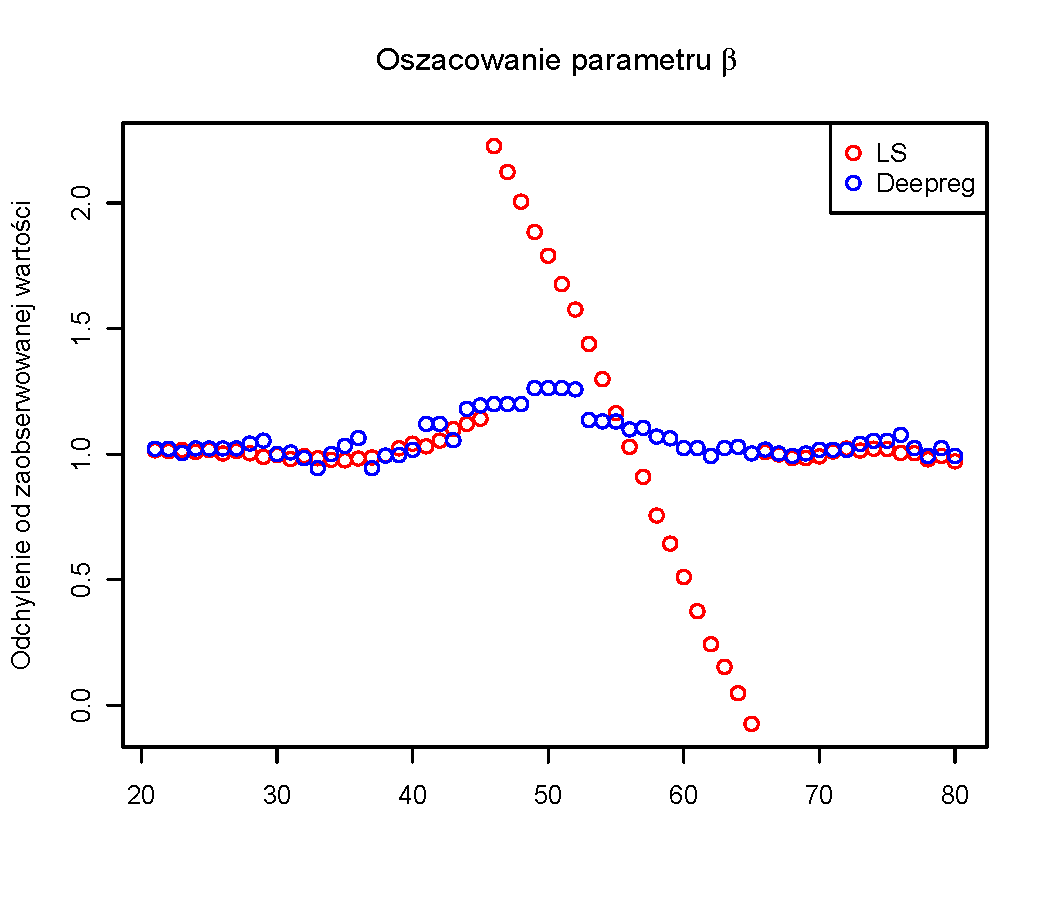
\includegraphics[width=\linewidth]{betaout}
  \caption{Oszacowanie parametru nachylenia}
  \label{fig:betaout}
\end{subfigure}
\caption{Oszacowania parametrów MNK i NGR w przypadku pojawienia się obserwacji odstającej}
\caption*{Źródło: Obliczenia własne - R Project}
\end{figure}

Rysunek \ref{fig:strepsilonout} przedstawia różnicę pomiędzy zaobserwowaną wartością a przewidywaną na podstawie poprzedniego okna. Obserwacja odstająca zaburza wskazania modelu MNK, aż do momentu, w którym zostaje wyłączona z okna. Z tego powodu błąd przez pewien okres kształtuje się na znacznie wyższym poziomie niż dla metody NGR.



\begin{figure}[h]
\centering
\vspace{-10pt}
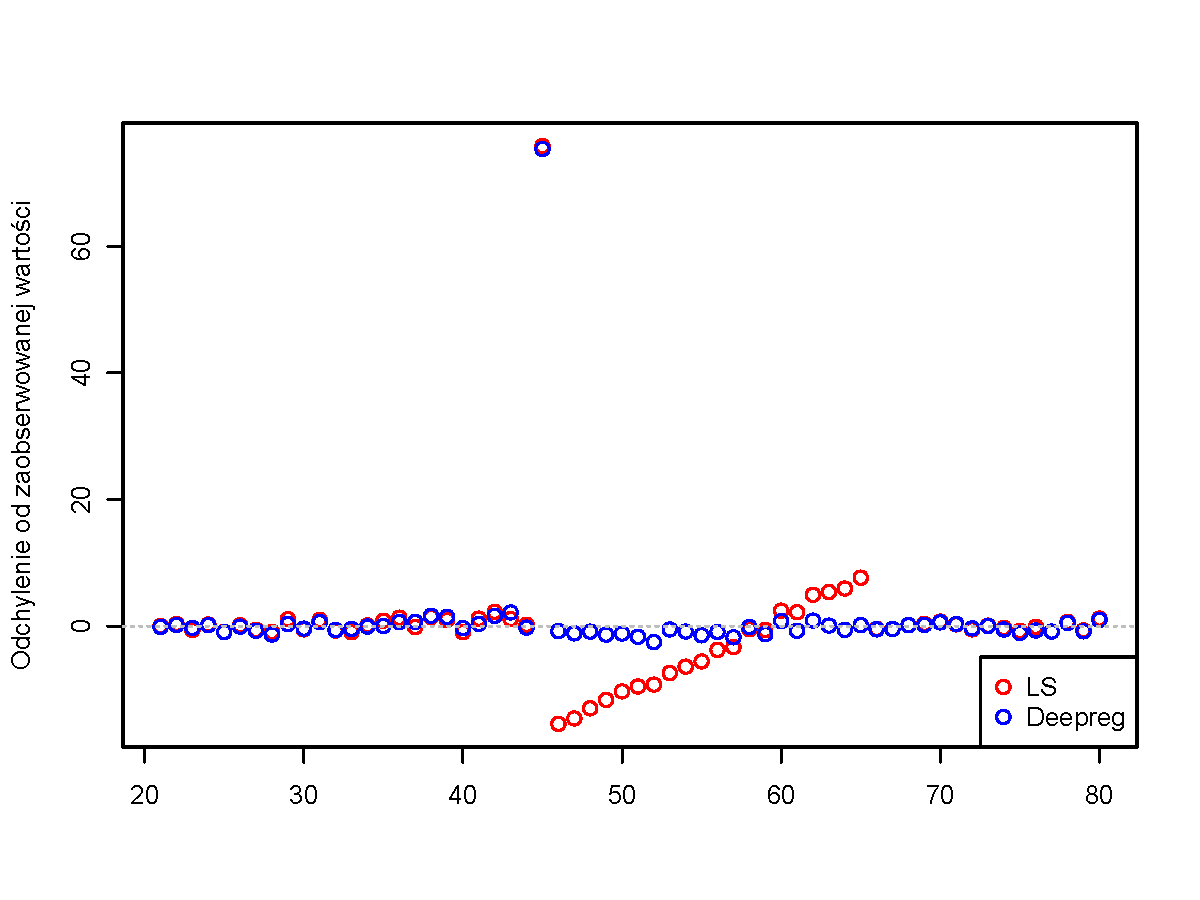
\includegraphics[width=80mm,height = 50mm]{strepsilonout}
\caption{Różnica pomiędzy przewidywaną obserwacją a zaobserwowaną w przypadku pojawienia się obserwacji odstającej}
\caption*{Źródło: Obliczenia własne - R Project}
\label{fig:strepsilonout}
\end{figure}

Należy zwrócić uwagę, iż w przypadku zmiany reżimu i obserwacji odstającej pojawienie się nowej obserwacji prowadziło do zmniejszenia się się błędu w przypadku MNK, natomiast dla NGR dla zmiany reżimu przez pewien czas odchylenie utrzymywało się na wysokim poziomie, a dla obserwacji odstającej na niskim i nie odbiegało od poprzednich wartości.

\chapter{Własności zaproponowanych metod}

\section{Analizowany problem}

Analizowanym problemem będzie przewidywanie warunkowej wartości oczekiwanej na podstawie okna $k$ ostatnich obserwacji, w przypadku strumienia danych o dwóch reżimach. Dodatkowo analizę przeprowadzono w przypadku występowania obserwacji odstających.


\section{Model analizowanego strumienia danych}

Jako model strumienia danych przyjęto proces CHARME\footnote{ang. Conditional Heteroscedastic Autoregressive Mixture of Experts}. CHARME jest to ogólna struktura do opisu szeregów czasowych ze zmiennymi reżimami, za które można przyjąć wiele procesów liniowych i nieliniowych, takich jak AR \footnote{ang. Autoregressive Model - model autoregresji}, GARCH\footnote{ang. Generalized Auto-Regressive Conditional Heteroskedasticity model - uogólniony model autoregresji z heteroskedastycznością warunkową}, czy  SV\footnote{ang. Stochastic Volatility - model wariancji stochastycznej}.

W modelu CHARME ukryty łańcuch Markowa ${Q_t}$ ze skończoną ilością stanów ${1,2,...,K}$ opisuje dynamikę kształtowania się procesu $X_t$ zdefiniowanego jako:
\begin{equation}
X_t = \sum^K_{k=1}S_{tk}(m_k(X_{t-1},...,X_{t-p})+\sigma ((X_{t-1},...,X_{t-p})\epsilon_t) + b_t\Theta,
\end{equation}
gdzie $S_{tk} = 1$ gdy $Q_t = k$ i $S_{tk} = 0$ w przeciwnym przypadku, oraz $m_k$, $\sigma_k$, $k = 1,..K$ to nieznane funkcje, $\epsilon \sim iid$ z wartością oczekiwaną równą 0, natomiast $b_t\Theta$ odpowiada za pojawianie się obserwacji odstających, $b_t$ jest nieobserwowalną zmienną losową o rozkładzie dwupunktowym, $\Theta$ jest obserwacją odstającą.

W badaniach symulacyjnych przyjęto dwa reżimy w postaci modeli $AR(1) \sim GARCH(1,1)$ o parametryzacji:
\begin{equation}
x_{t+1} = \mu + \theta x_{t} + Z_t,
\end{equation}
\begin{equation}
Z_t = \sigma_t \epsilon_t,
\end{equation}
\begin{equation}
\sigma_t^2 = c_0+ \alpha Z_{t-1} + \beta \sigma_{t-1}.
\end{equation}
Parametry modelu:
 
Reżim 1:
$\mu = 2$, $\theta = 0.8$, $c_0 = 0.1$ ,$\alpha = 0.1$, $\beta = 0.75$,

Reżim 2:
$\mu = -0.5$, $\theta = 0.2$, $c_0 = 0.1$, $\alpha = 0.6$, $\beta = 0.1$.

W obu przypadkach $\epsilon_t$ to rozkład t-studenta o czterech stopniach swobody. 

Rysunki \ref{fig:simex} i Rysunki \ref{fig:simexout} przedstawiają przykładowe trajektorie procesu CHARME zdefiniowanego w powyższy sposób.

\begin{figure}[H]
\centering
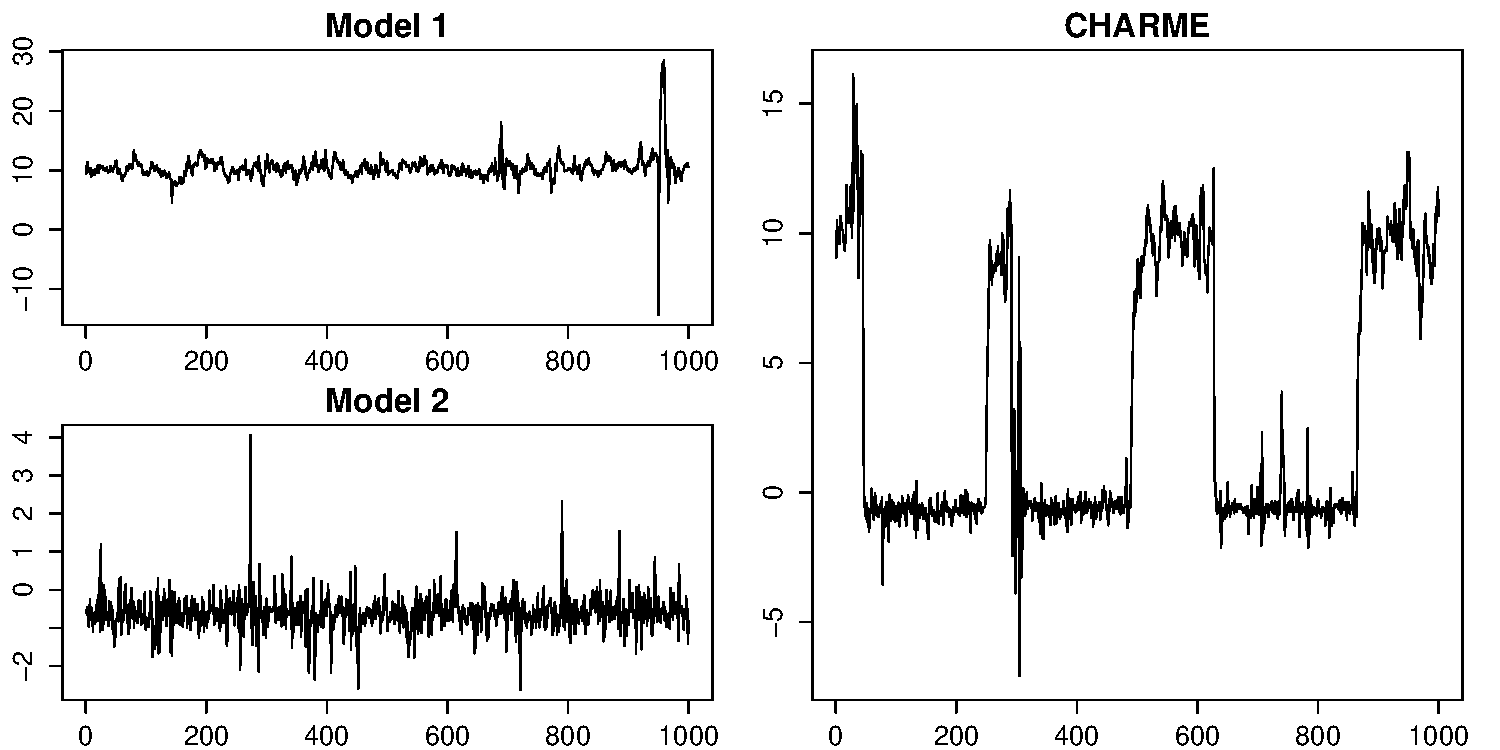
\includegraphics[width=160mm,height = 60mm]{simex}
\caption{Przykładowe trajektorie dla procesów wchodzących w skład analizowanego modelu CHARME i samego modelu bez obserwacji odstających}
\caption*{Źródło: Obliczenia własne - R Project}
\label{fig:simex}
\end{figure}

\begin{figure}[H]
\centering
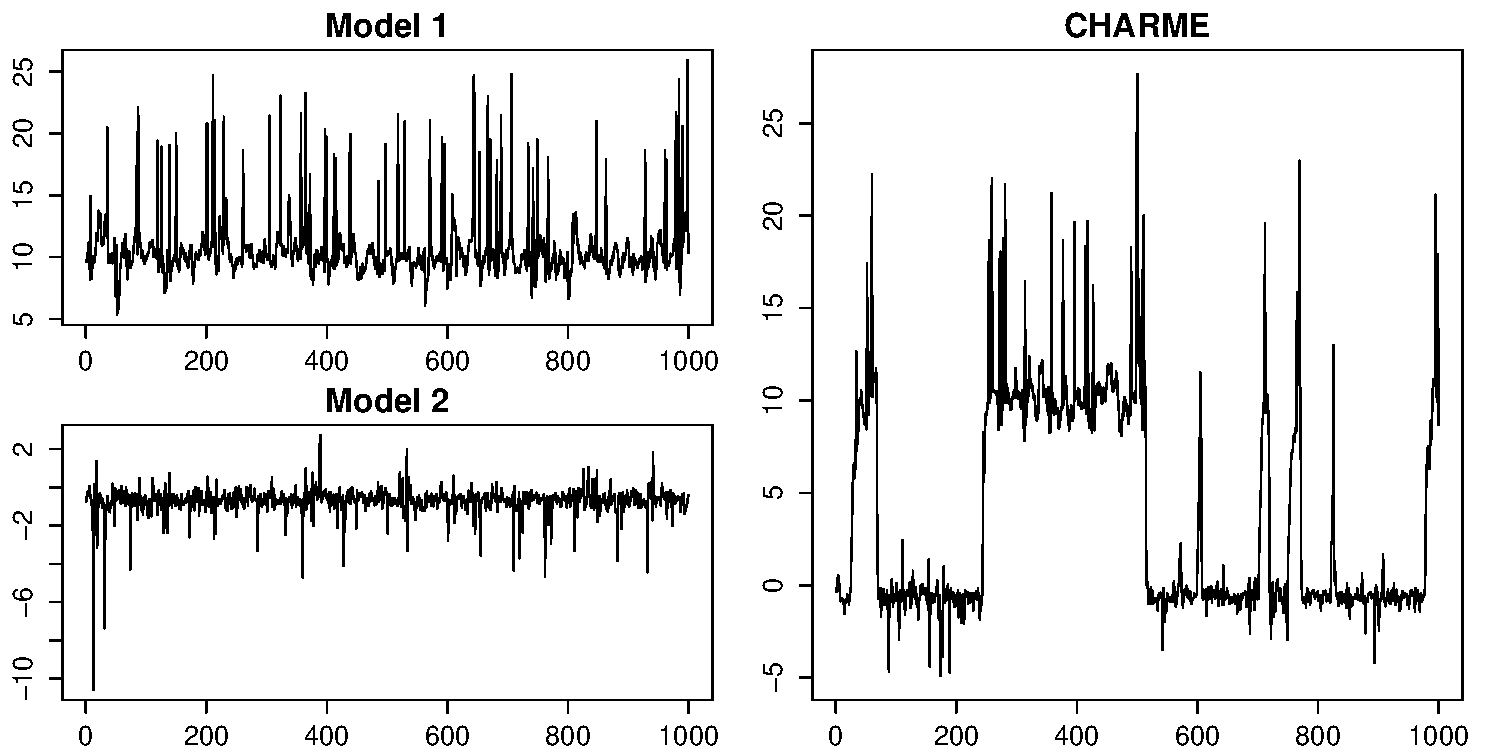
\includegraphics[width=160mm,height = 60mm]{simexout}
\caption{Przykładowe trajektorie dla procesów wchodzących w skład analizowanego modelu CHARME i samego modelu z obserwacjami odstającymi (5\%)}
\caption*{Źródło: Obliczenia własne - R Project}
\label{fig:simexout}
\end{figure}


\section{Wyniki symulacji w przypadku braku występowania obserwacji odstających}

W tabeli \ref{restable} zebrano parametry oceniające jakość użytych modeli. Zostały one wyznaczone symulacyjne na podstawie 500 trajektorii modelu CHARME.

Zdefiniowane zostały jako: 

\begin{equation}
RMSE = \frac{\sum_{t=s}^{T}({E}(x_{t}|\Psi_{t-1})-\hat{E}(x_{t}|W_{t-1,k}))^2}{T-s},
\end{equation}

\begin{equation}
ME = \frac{\sum_{t=s}^{T}({E}(x_{t}|\Psi_{t-1})-\hat{E}(x_{t}|W_{t-1,k}))}{T-s},
\end{equation}

\begin{equation}
MAE = \frac{\sum_{t=s}^{T}|{E}(x_{t}|\Psi_{t-1})-\hat{E}(x_{t}|W_{t-1,k})|}{T-s},
\end{equation}

\begin{equation}
max(\hat{\epsilon}) = max_{t \in (s,...,T)}({E}(x_{t}|\Psi_{t-1})-\hat{E}(x_{t}|W_{t-1,k})),
\end{equation}

\begin{equation}
min(\hat{\epsilon}) = min_{t \in (s,...,T)}({E}(x_{t}|\Psi_{t-1})-\hat{E}(x_{t}|W_{t-1,k})),
\end{equation}

gdzie:

\begin{itemize}
\item $T$ - ilość obserwacji w szeregu. W symulacjach $T=1000$.
\item $s$ - moment w którym wyznaczono pierwszą prognozę, wcześniejsze obserwacje zostały użyte jako pierwsze okno do wyznaczania modelu. W symulacjach $s = 101$.
\item $\Psi_{t}$ - historia procesu do chwili $t$.
\item $W_{t,k}$ - okno danych, $k$ oznacza długość okna, w symulacjach $k=100$.
\item ${E}(x_{t}|\Psi_{t-1})$ - wartość oczekiwana warunkowa procesu w chwili $t$ wyznaczona analitycznie na podstawie parametrów reżimu w którym proces aktualnie się znajdował.
\item $\hat{E}(x_{t}|W_{t-1,k})$ - prognoza wartości oczekiwanej warunkowa w chwili $t$ wyznaczona na podstawie okna $W_{t-1,k}$.
\end{itemize}


Najlepszą metodą okazała się regresja najmniejszych kwadratów. Należy jednak zwrócić uwagę na to, że również w jej przypadku nastąpiły największe odchylenia od prawdziwej wartości oczekiwanej warunkowej. 

\begin{table}[H]
\caption{Podstawowe parametry oceniające jakość użytych modeli}
\label{restable}
\begin{tabular}{|r|l|l|l|l|l|}
  \hline
  Metoda & RMSE & ME & MAE & $max(\hat{\epsilon})$& $min(\hat{\epsilon})$ \\
  \hline 
  Najmniejsze kwadraty & 0.501 & 0.0112 & 0.253 & 19.63 & -21.994\\
  \hline
  Metoda NGR & 1.099 & 0.1665 & 0.430 & 15.67 & -14.673\\
  \hline
  KNN(5) - Euklides & 0.8577 & 0.0534 & 0.385 & 14.12 & -11.29\\
  \hline
  
\end{tabular}
\caption*{Źródło: Obliczenia własne - R Project}
\end{table}


W dalszej analizie zbadano zachowanie się poszczególnych algorytmów w momencie zmiany reżimu. Na poniższym wykresie \ref{odch1} szarą pionową linią zaznaczono moment zmiany reżimu.

\begin{figure}[H]
\centering
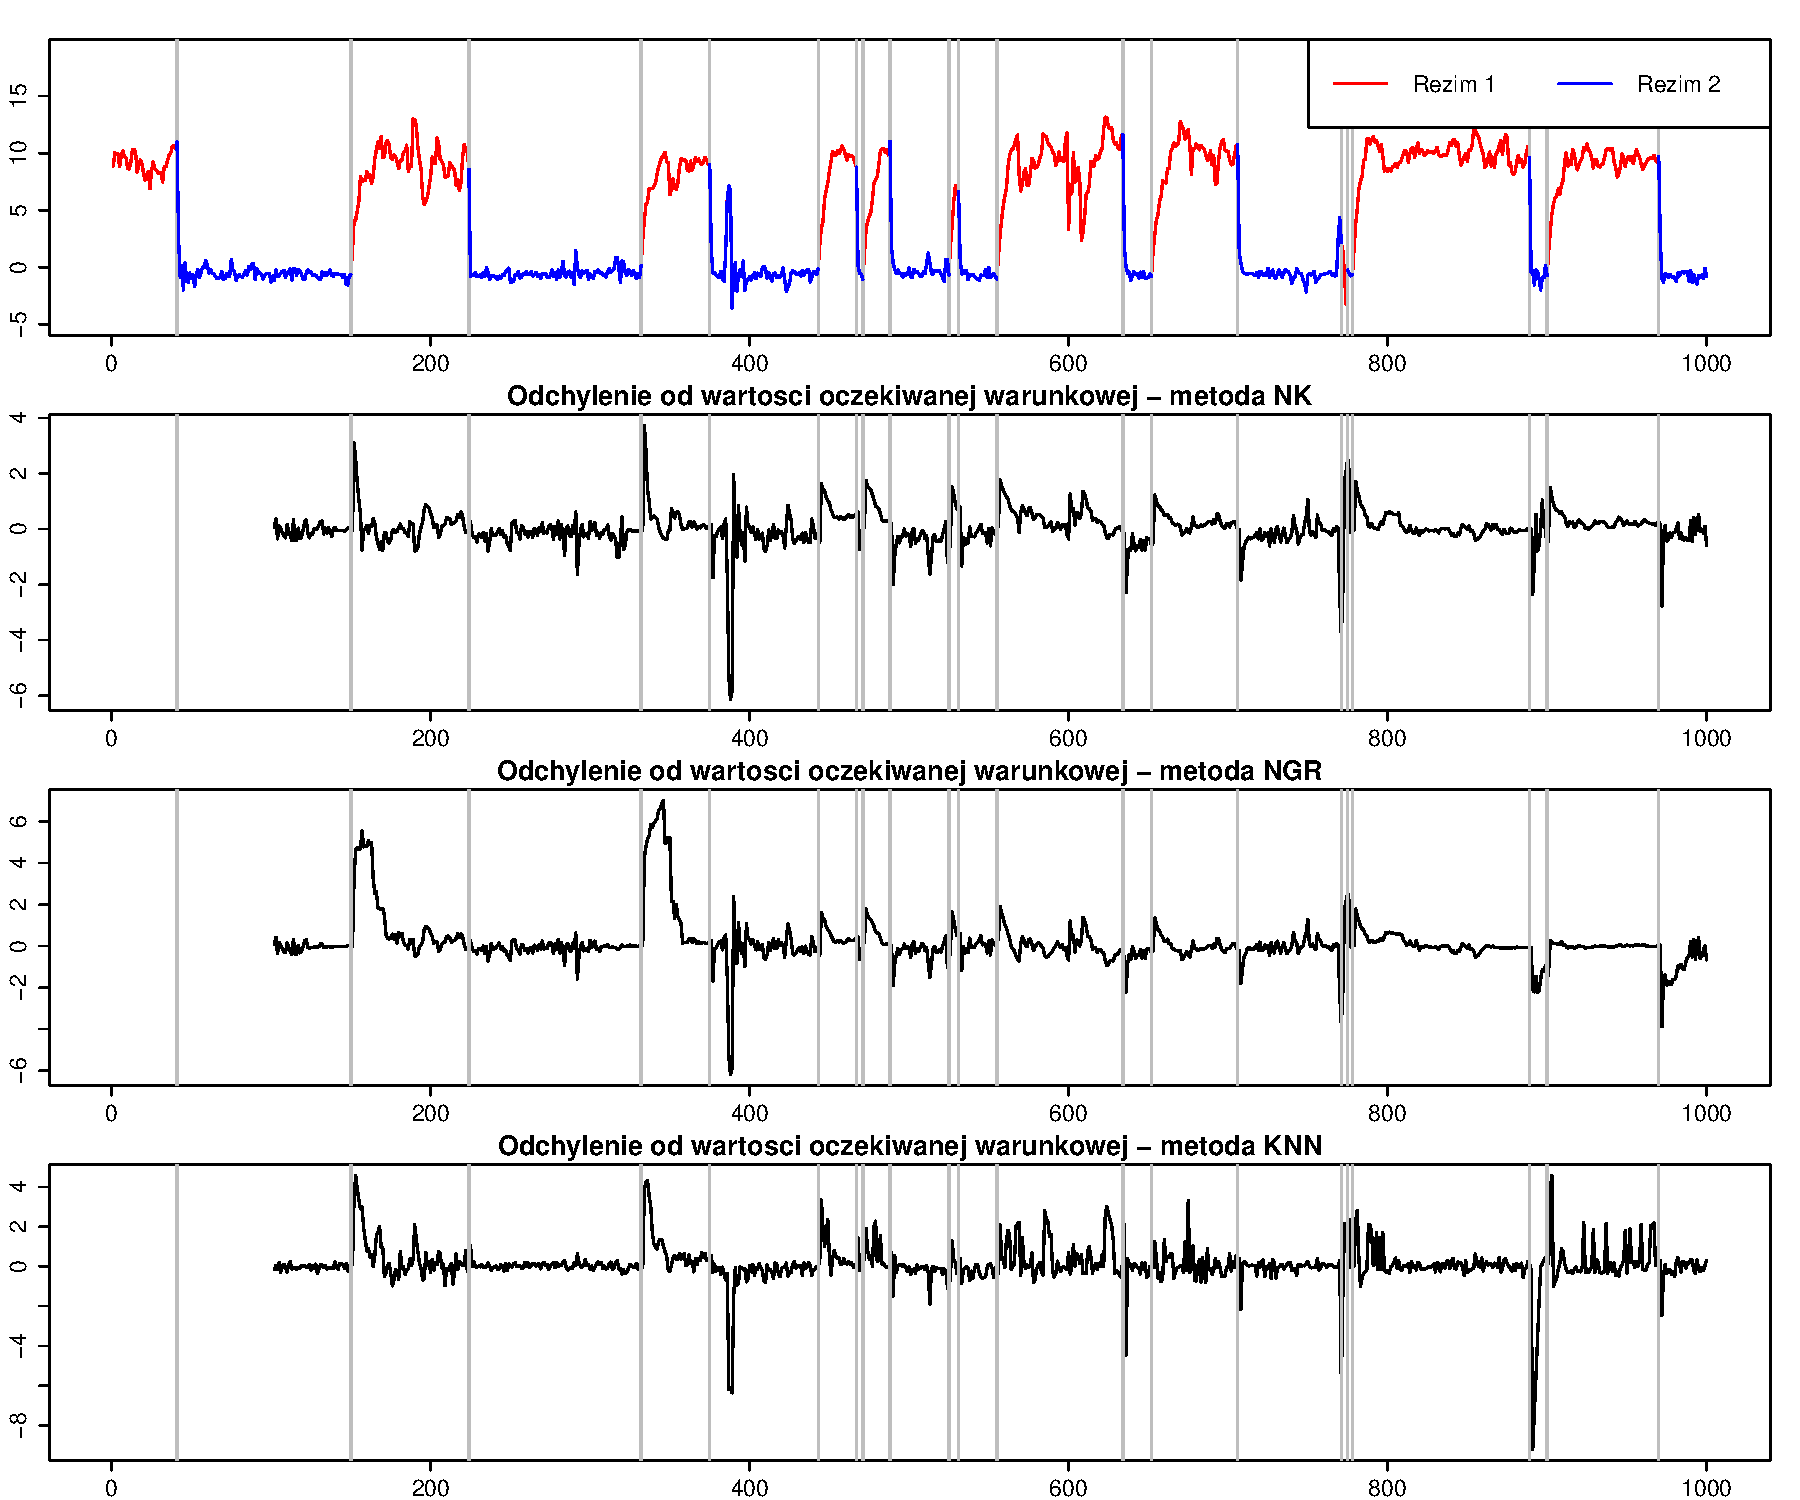
\includegraphics[width=160mm,height = 120mm]{compreg}
\caption{Odchylenia od wartości oczekiwanej warunkowej dla przykładowej trajektorii modelu CHARME}
\caption*{Źródło: Obliczenia własne - R Project}
\label{odch1}
\end{figure}


W powyższym przypadku można zaobserwować zjawisko opisane w \ref{s:lab}. Otóż przez pewien okres, po zmianie reżimu w przypadku regresji NGR pojawiające się obserwacje traktowane były jako odstające, przez co, wskazania były bardziej związane z poprzednim reżimem niż z nowym. Natomiast regresje nieodporne znacznie szybciej przesunęły się w stronę nowego reżimu. Obserwacja ta sugeruje, iż w przypadku regresji na oknie danych dla procesu o zmiennych reżimach, przy braku występujących obserwacji odstających powinno raczej używać się metod nieodpornych, gdyż są one w stanie szybciej przejść ze starego reżimu do nowego. Na wykresie \ref{fig:odchreg} przedstawiono fragment przykładowej trajektorii procesu CHARME w momencie zmiany reżimu, wraz z krzywymi przedstawiającymi predykcję wartości oczekiwanej wyznaczoną na podstawie poprzedzającego ją okna.

\begin{figure}[H]
\centering
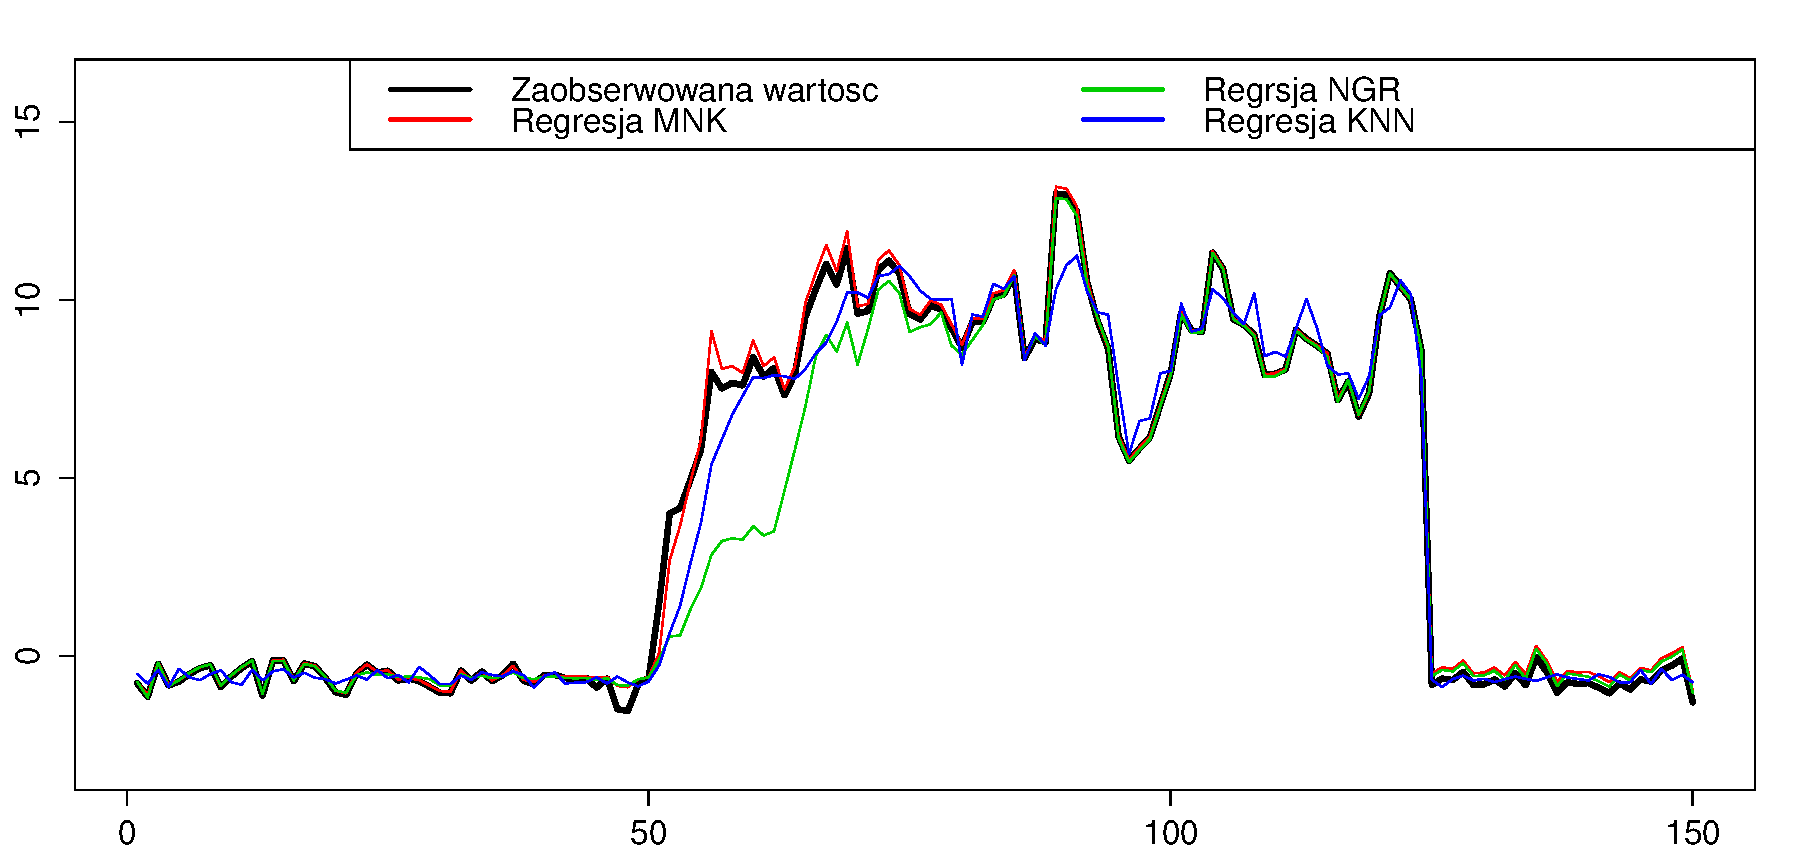
\includegraphics[width=160mm,height = 60mm]{esval}
\caption{Zestawienie wartości przewidywanych na podstawie ostatniego okna i faktycznej trajektorii procesu.}
\caption*{Źródło: Obliczenia własne - R Project}
\label{fig:odchreg}
\end{figure}

\section{Wyniki symulacji w przypadku występowania obserwacji odstających}

W tabeli \ref{restableout}  zebrano podstawowe parametry oceniające jakość użytych modeli. W przypadku występowania obserwacji odstających najlepszym estymatorem wartości oczekiwanej warunkowej okazała się metoda największej głębi regresyjnej. Wzrost błędu predykcji spowodowany późniejszą reakcją na zmianę reżimu miał znacznie mniejsze znaczenie dla oszacowania niż pojawiające się obserwacje odstające.

\begin{table}[H]
\caption{Podstawowe parametry oceniające jakość użytych metod w przypadku występowania obserwacji odstających}
\label{restableout}

\begin{tabular}{|r|l|l|l|l|l|}
  \hline
  Metoda & RMSE & ME & MAE & $max(\hat{\epsilon})$& $min(\hat{\epsilon})$ \\
  \hline 
  Najmniejsze kwadraty & 5.011 & -0.490 & 2.759 & 131.32 & -232.525\\
  \hline
  Metoda NGR & 2.133 & 0.252 & 0.800 & 74.904 & -85.286\\
  \hline
  KNN(5) - Euklides & 6.041 & -0.110 & 2.435 & 121.299 & -46.15\\
  \hline
\end{tabular} 
\end{table}

Rysunek \ref{fig:outcharme} przedstawia kształtowanie się odchyleń od wartości oczekiwanej przy założeniu pojawiania się obserwacji odstających.

\begin{figure}[H]
\centering
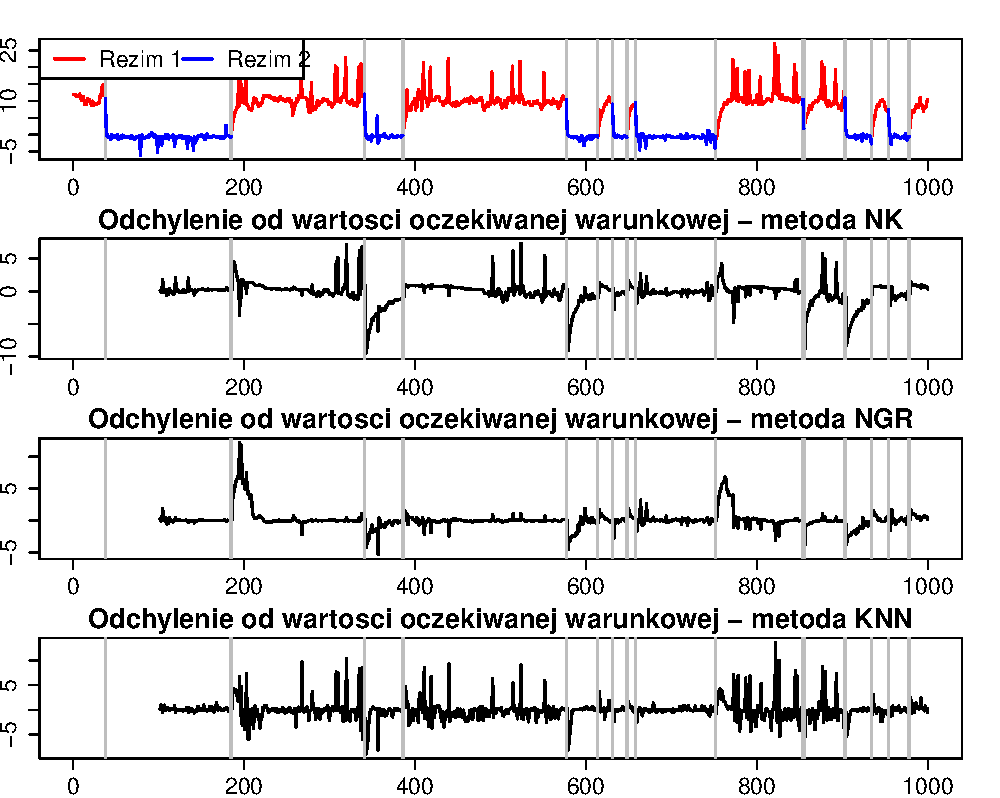
\includegraphics[width=160mm,height = 120mm]{outcharme}
\caption{Odchylenia od wartości oczekiwanej warunkowej dla przykładowej trajektorii modelu CHARME}
\caption*{Źródło: Obliczenia własne - R Project}
\label{fig:outcharme}
\end{figure}


\section{Długość okna}

W przypadku analizy strumienia danych przy pomocy okna należy ustalić jego długość. W tym kontekście pojawia się dylemat, czy ustalone okno ma być krótkie tak, by uwzględniać jedynie najbardziej aktualny stan strumienia, czy przeciwnie - powinno być długie, by lepiej lepiej reprezentować strumień w okresie stabilności. W dalszej części przeprowadzono analizę  porównawczą omawianych algorytmów z uwagi na długość okna danych. Dla algorytmu KNN ilość najbliższych sąsiadów wyznaczana była jako jedna dziesiąta długości okna. Na rysunku \ref{fig:window} przedstawiono średni błąd RMSE w zależności od długości okna.

\begin{figure}[H]
\centering
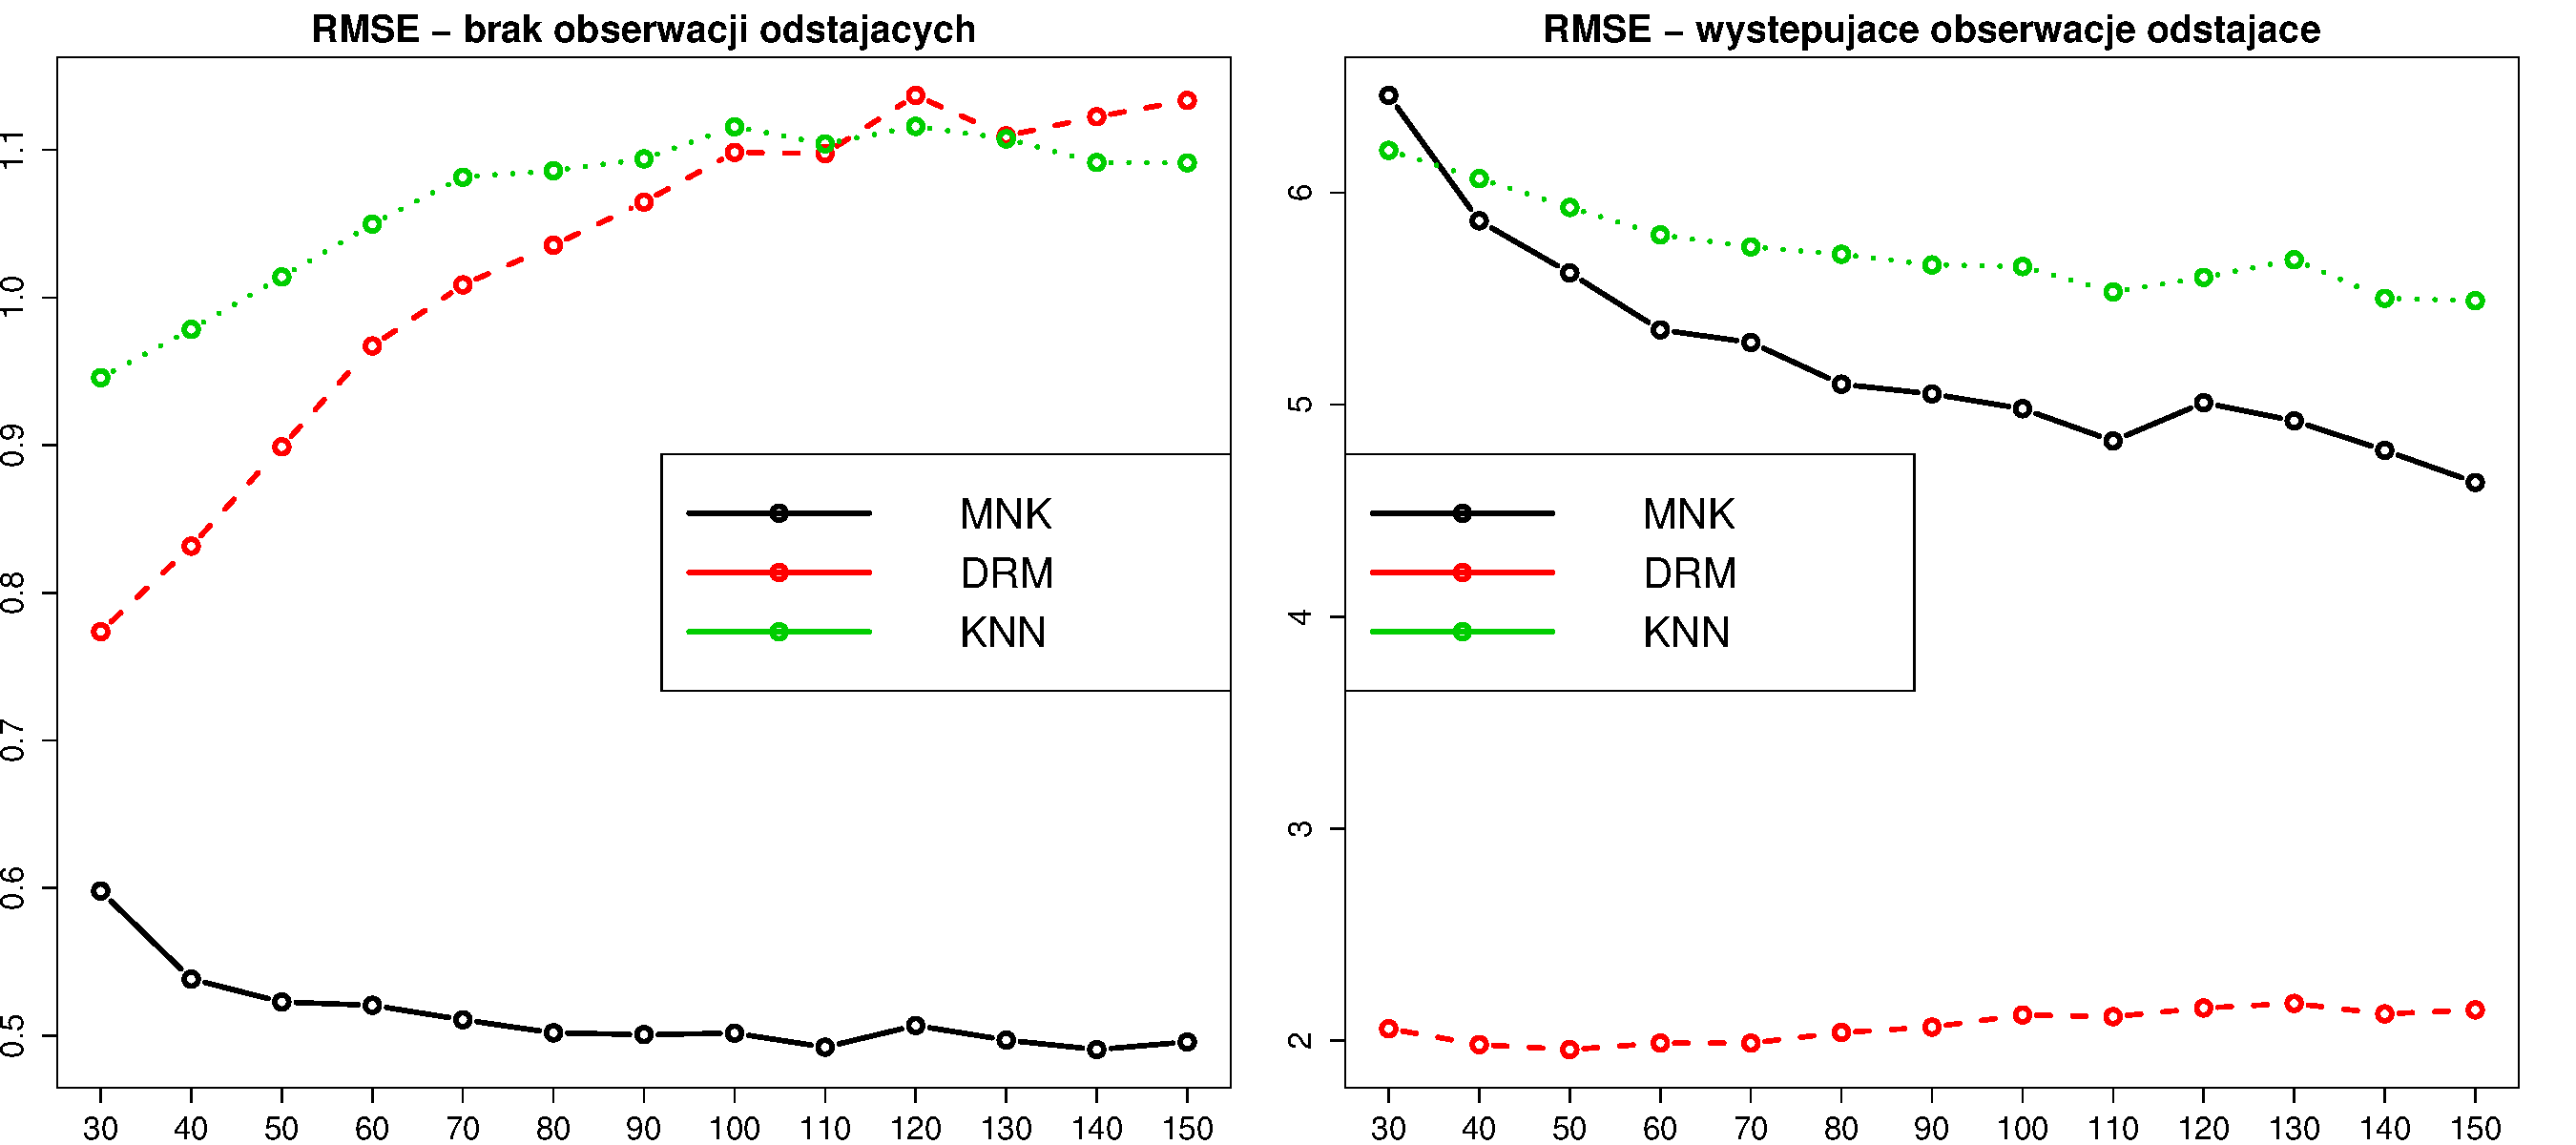
\includegraphics[width=160mm,height = 60mm]{rmse}
\caption{RMSE dla modeli dla różnych długości okna}
\caption*{Źródło: Obliczenia własne - R Project}
\label{fig:window}
\end{figure}

W przypadku braku obserwacji odstających, dla regresji MNK rozmiar okna nie miał kluczowego znaczenia - dla rozmiaru powyżej 70 obserwacji błąd utrzymywał się na zbliżonym poziomie, jednak w przypadku regresji metodą największej głębi regresyjnej im okno było krótsze tym odchylenie od zaobserwowanych wartości było mniejsze. W przypadku występowania obserwacji odstających dla metody NGR wybór długości okna nie wpływał znacząco na oszacowania, natomiast dla regresji MNK wraz z wydłużeniem się okna błąd malał.

\mgrclosechapter



\chapter{Przykład empiryczny - RegTrend - prosta strategia typu Trend Following}

W dzisiejszym świecie bardzo dużą rolę w handlu giełdowym odgrywa handel algorytmiczny. Decyzja o kupnie lub sprzedaży określonego aktywa zostaje podjęta na bazie określonej strategii inwestycyjnej z wyłączeniem udziału człowieka. W takim podejściu możliwe jest monitorowanie dziesiątek tysięcy aktywów z różnych giełd światowych i wyszukiwanie okazji do transakcji, których człowiek nie jest w stanie dostrzec.

Jako przykład zastosowania modelu strumienia danych i prostej regresji dla handlu algorytmicznego skonstruowano prostą strategię typu Trend Following \footnote{Trend Following - strategia mająca na celu podążanie za trendem w którym aktualnie znajduje się dany instrument}, wykorzystującą regresję na oknie. Strategii nadano nazwę RegTrend. Następnie przeprowadzono proces sprawdzania jej użyteczności.

\section{Opracowanie sygnału generującego zdarzenie}

Pierwszym etapem w tworzeniu strategii algorytmicznej jest przygotowanie sygnału (lub zestawu), który będzie określał jakie działanie ma zostać podjęte. Poniżej znajduje się lista przykładowych operacji:

\begin{itemize}
\item zajęcie pozycji na aktywie - czy w danym momencie należy kupić (zająć długą pozycję) lub sprzedać (zająć krótką pozycję) dany aktyw, lub koszyk aktywów ,
\item Stop Loss - czy należy w danym momencie zamknąć pozycję z powodu, że aktualna strata przekracza ustalony wcześniej poziom,
\item Take Profit - czy zamknąć pozycję, gdyż został osiągnięty oczekiwany zysk,
\item powiększenie pozycji - czy należy powiększyć daną pozycję na aktywie.
\end{itemize}

W przypadku analizowanej strategii RegTrend, sygnał otwarcia pozycji opierał się na współczynniku nachylenia regresji na oknie ostatnich $40$ cen zamknięcia dla danego instrumentu. Jeżeli był on dodatni zajmowana zostawała była pozycja długa (dany aktyw był kupowany), jeżeli ujemny - krótka (sprzedaż aktywa). W przypadku zmiany znaku tego współczynnika pozycja była obracana (przejście z pozycji krótkiej na długą i odwrotnie). Do zamykania pozycji zastosowano również mechanizm Trailing Stop polegający na tym, że w przypadku zmiany ceny korzystnej ze względu na zajętą pozycję, poziom na jakim zostaje wykonane zlecenie stop loss podnosi się. Pozwala to zachować osiągnięty zysk, w przypadku możliwych dalszych niekorzystnych zmian na rynku. Stop Loss został ustawiony na poziomie 5\%. 

W przypadku wystąpienia zlecenia Stop Loss chwilowo zostawało także skracane okno na jakim była wyznaczana regresja do 10 ostatnich obserwacji. Wynika to z przekonania autora, że w przypadku, gdy zajęta pozycja przynosi dużą stratę, w ostatnim krótkim czasie nastąpiła gwałtowna zmiana sytuacji rynkowej (np. głębokie załamanie). Należy więc ograniczyć się do ostatniej, znacznie krótszej historii.

Dodatkowym mechanizmem ograniczającym ostateczną możliwą stratę jest wyłączanie strategii w przypadku, gdy aktualny  kapitał spadł do poziomu poniżej 80\% kapitału początkowego. To podejście ma na celu ujęcie w pewien sposób faktu, że o ile w przypadku testu na danych historycznych widzi się całą trajektorię przedstawiającą wynik strategii, to dla aktualnych danych dalsza trajektoria nie jest znana, a wraz z rosnącą stratą rośnie przekonanie, że należy interweniować manualnie i taką strategię wyłączyć. Ma to również znaczenie w przypadku funduszy inwestycyjnych i budowania "track record'u", czyli historii wyniku finansowego. Jeżeli w początkowym okresie fundusz zrealizował dużą stratę ma mniejsze szanse na znalezienie kolejnych inwestorów.

\section{Backtest - analiza wyników}

Następnym etapem analizy strategii jest przeprowadzenie ,,backtestu''. Polega on na zastosowaniu danej strategii na danych historycznych dla określonej grupy aktywów. Jako porównanie dla RegTrend przyjęto strategię ,,Buy-and-hold''\footnote{ang. Buy and Hold - Kup i Trzymaj} polegającą na zakupie danego aktywa na początku okresu i sprzedaży na końcu. 

Rysunek \ref{fig:google} przedstawia wyniki strategii dla spółki Google. Wykres zawiera trzy krzywe:
\begin{description}
\item [Balance] - jest to stan środków na koncie w danej chwili wraz z wartością otwartych pozycji po cenie otwarcia liczone według wzoru \ref{e:bal},
\item [Equity] - jest to aktualny balans skorygowany o aktualne zyski bądź straty na pozycjach. Krzywa equity prezentuje stan środków, jaki znalazłby się na koncie, jeśli w danej chwili zostałyby zamknięte wszystkie otwarte pozycje po aktualnej cenie rynkowej. Krzywa Equity została wyznaczona na podstawie wzoru \ref{e:equity}.
\item [Buy-and-hold] - przedstawia krzywą Equity dla strategii ,,Buy-and-hold''.
\end{description}
\begin{equation}\label{e:bal}
B_t = K_0 + \sum_{i=1}^NR_i,
\end{equation}
gdzie $K_0$ to kapitał początkowy, $N$ to ilość zamkniętych pozycji, to chwili $t$ włącznie, natomiast $R_i$ to zysk z i-tej pozycji obliczany według formuły \ref{e:long} dla długiej pozycji lub \ref{e:short} dla pozycji krótkiej.
\begin{equation}\label{e:long}
R_i = (P_c(1-C) - P_o(1+C)) \cdot \frac{K_o}{P_o(1+C)},
\end{equation}
\begin{equation}\label{e:short}
R_i = (P_o(1-C) - P_c(1+C) \cdot \frac{K_o}{P_o(1+C)},
\end{equation}
gdzie $P_o$, to cena zamknięcia dla instrumentu finansowego w dniu w którym wystąpił sygnał otwarcia pozycji, natomiast $P_c$, to cena instrumentu w dniu w którym pozycja została zamknięta. $C$ jest to wysokość prowizji, w tym przypadku wynosi ona $0.02\%$. $K_o$ to wolne środki pieniężne w chwili w dniu otwarcia pozycji, iloraz $\frac{K_o}{P_o(1+C)}$ oznacza zrealizowany wolumen w chwili otwarcia (dopuszczalne są części ułamkowe akcji).

\begin{equation}\label{e:equity}
E_t = B_t + PnL_t,
\end{equation}
gdzie $E_t$ to wartość Equity w chwili $t$, $B_t$ wartość Balance wyznaczona ze wzoru \ref{e:bal}, $PnL_t$ - niezrealizowany zysk lub strata z otwartej pozycji w chwili $t$. Jeżeli nie ma otwartej żadnej pozycji wtedy $B_t=E_t$.

Wartości Balance, Equity dla RegTrend i ,,Buy and Hold'' wyznaczone ze wzorów \ref{e:bal} i \ref{e:equity} wyrażone są w pieniądzu. By ułatwić interpretację wykresów i uniezależnić przedstawione wyniki od kapitału początkowego wartości te zostały przeskalowane według wzoru \ref{e:skal}, by przedstawiały procentowa zmiana względem kapitału początkowego przeznaczonego na strategię.
\begin{equation}\label{e:skal}
S_t\% = \frac{L_t}{K_0}-1,
\end{equation}
gdzie $L_t$ to wartość  Balance lub Equity w chwili $t$, natomiast $K_0$ to kapitał początkowy przeznaczony na strategię.

W tym przypadku strategia daje wyniki zbliżone do strategii ,,Buy and Hold''.
\begin{figure}[H]
\centering
\vspace{-10pt}
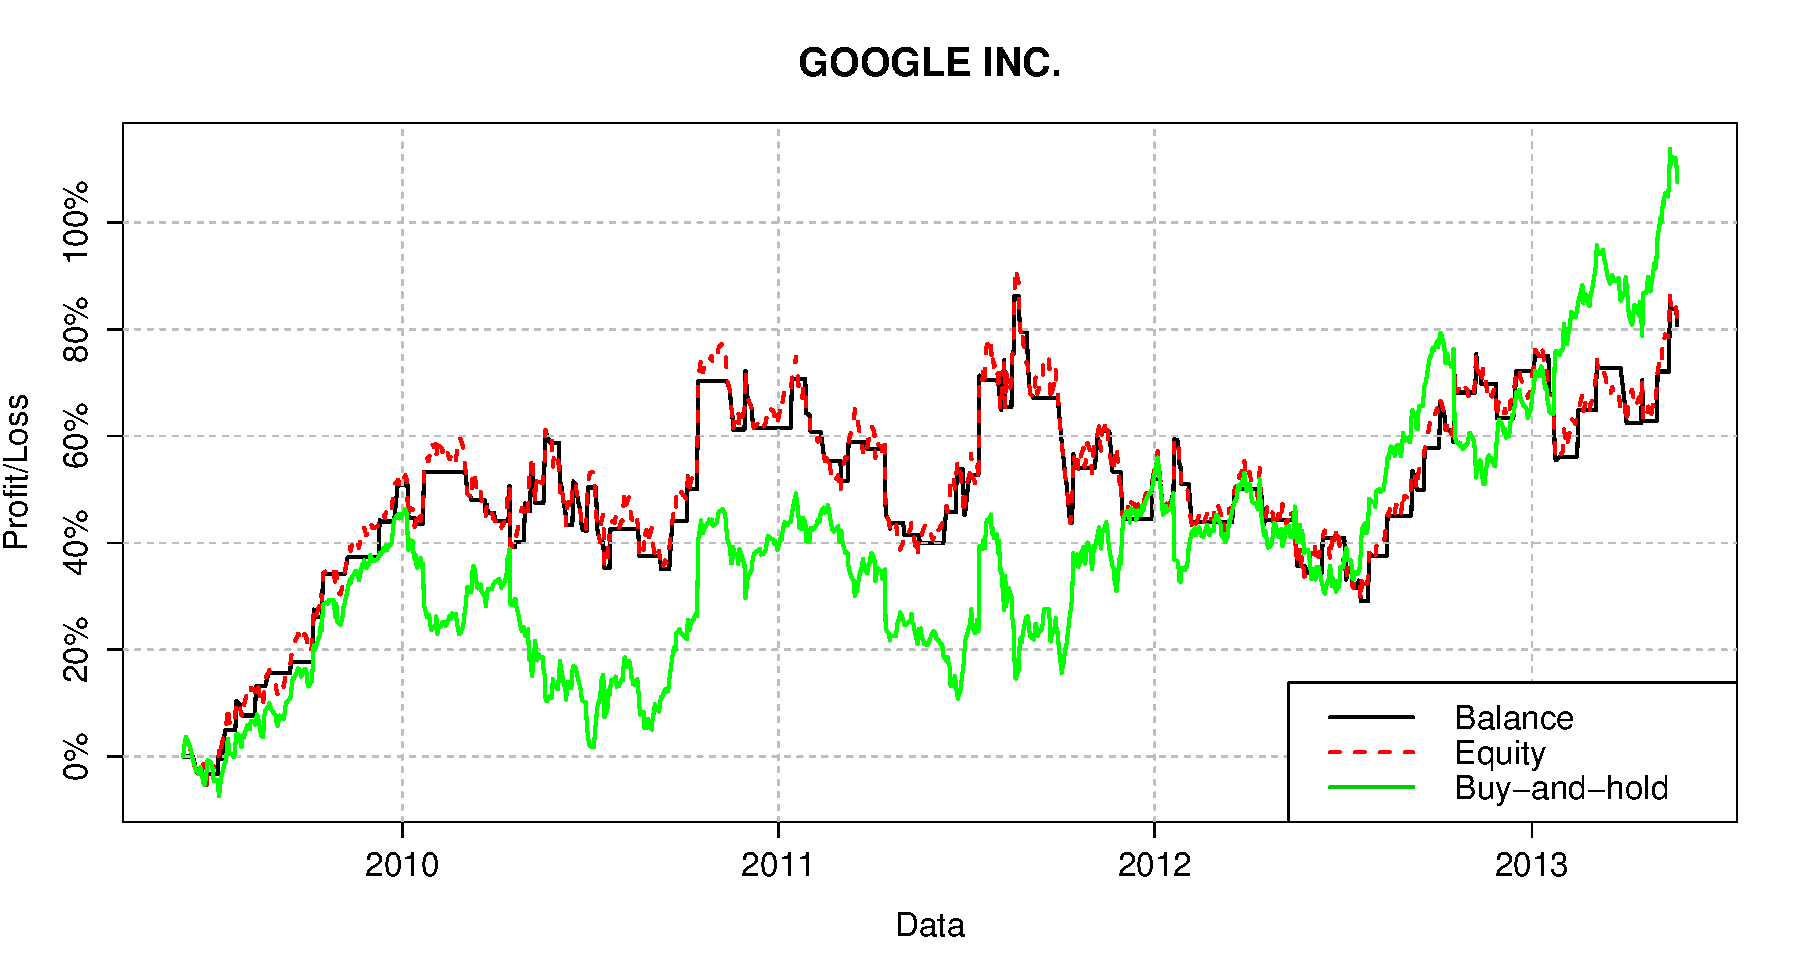
\includegraphics[width=120mm,height = 60mm]{google}\vspace{-10pt}
\caption{Krzywe Balance, Equity dla strategii RegTrend zostosowanej dla spółki Google, porównane ze strategią ,,Buy-and-hold''}
\caption*{Źródło: Obliczenia własne - R Project}
\label{fig:google}\vspace{-10pt}
\end{figure}

W dalszej części przeprowadzono analizę dla szerszego spektrum aktywów (2093 instrumentów pochodzące z NASDAQ). Wymaganiem by dany aktyw został dołączony do testu był jedynie fakt, czy posiada on wystarczająco długą historię (czy był notowany od dnia 6 maja 2009 roku, do 22 maja 2013). Poniżej przedstawiono wykres (rys. \ref{fig:allmarket})  analogiczny jak w przypadku wyniku strategii dla spółki Google. Prezentuje on sumaryczny wynik dla strategii dla całej gamy aktywów. Wartości Balance i Equity w przypadku portfela aktywów została wyznaczona na podstawie wzorów \ref{e:pbal} i \ref{e:peq}.
\begin{equation}\label{e:pbal}
B_t = \sum_{j = 1}^M(K_{j,0} + \sum_{i=1}^{N_j}R_{ji}),
\end{equation}
\begin{equation}\label{e:peq}
E_t = B_t + \sum_{j = 1}^MPnL_{jt},
\end{equation}
gdzie $M$ to ilość aktywów w portfelu (w analizowanym przypadku $M=2093$), inne oznaczenia są analogiczne jak w przypadku \ref{e:bal} i \ref{e:equity}, z tą różnicą, że odnoszą się do wartości związanych z j-otym instrumentem, Dla każdego instrumentu kapitał początkowy był równy ($K_{1,0}=K_{2,0}=K_{M,0}$). Również wartości Equity i Balance zostały przeskalowane podobnie jak w przypadku \ref{e:skal}.
\begin{figure}[H]
\centering
\vspace{-10pt}
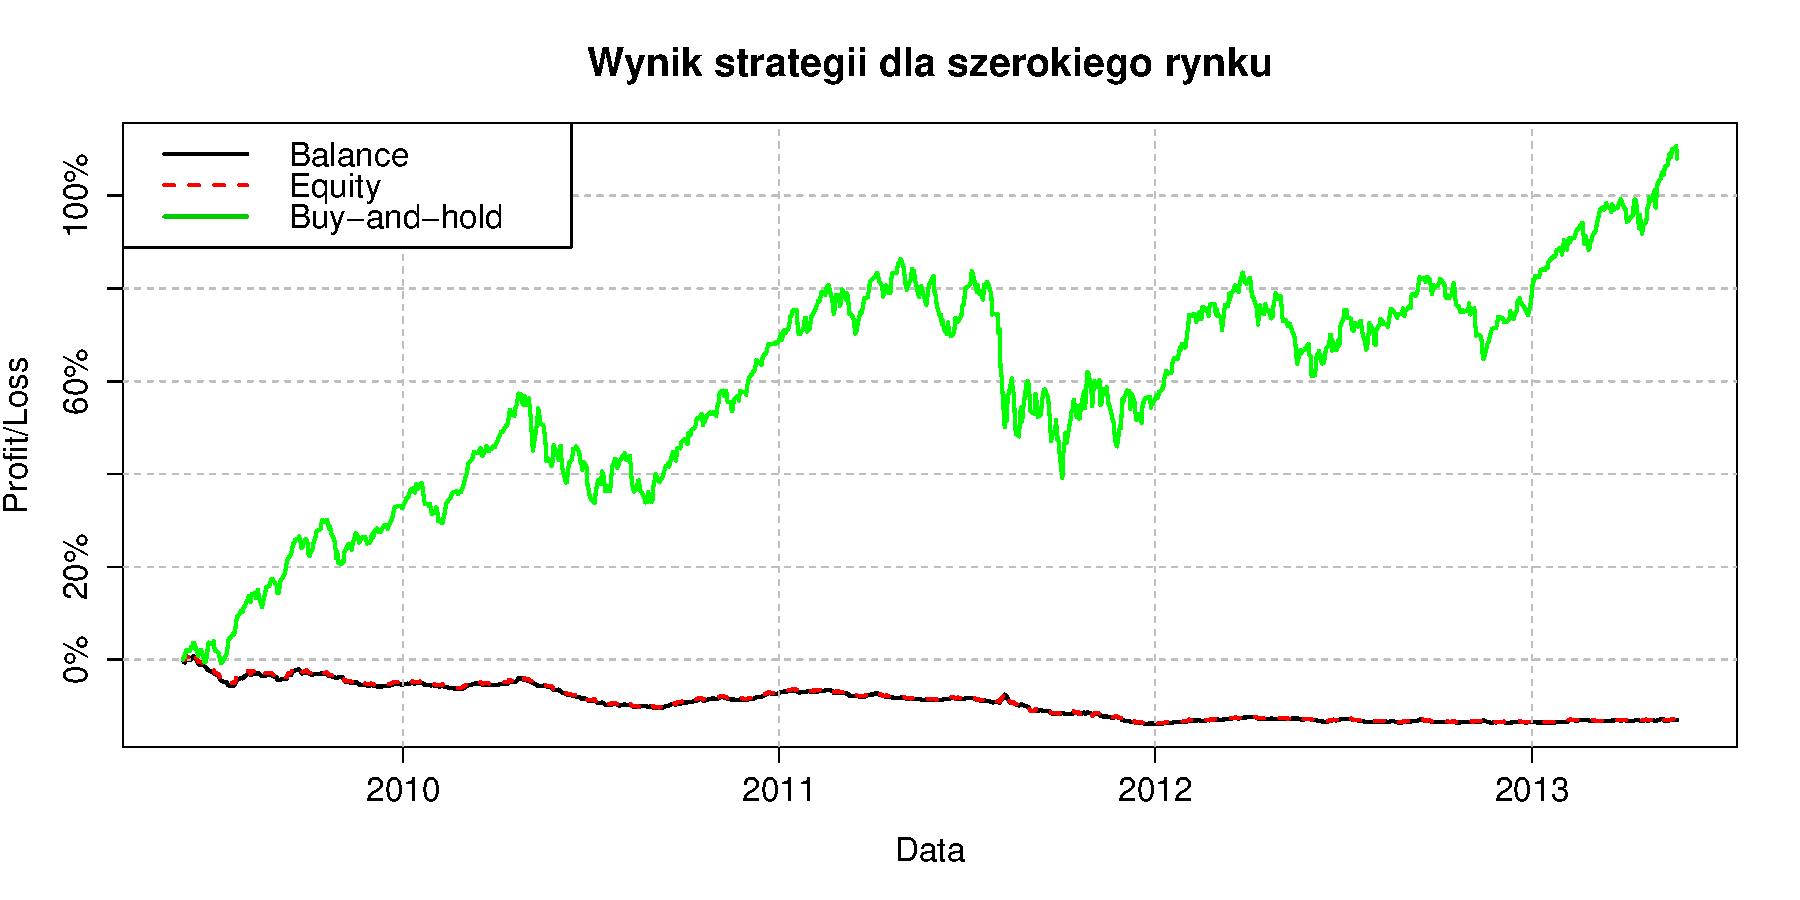
\includegraphics[width=110mm,height = 60mm]{allmarket}
\vspace{-10pt}
\caption{Krzywe Balance, Equity dla strategii RegTrend zastosowanej dla szerokiego rynku, porównane ze strategią ,,Buy-and-hold''.}\vspace{-12pt}
\caption*{Źródło: Obliczenia własne - R Project}
\label{fig:allmarket}\vspace{-12pt}
\end{figure}

Dla zestawu aktywów RegTrend okazał się znacznie gorszy od prostej strategii "Buy-and-hold". W analizowanym okresie, przy założeniu, że w każdy aktyw inwestowana byłaby taka sama kwota, RegTrend przyniósłby 13\% stratę (3.42\% średniorocznie), natomiast ,,Buy-and-hold'' zarobiłby 108\% (20.1\% średniorocznie).

Przypadek, w którym strategia systematycznie traci (krzywa Balance jest nachylona ujemnie) oznacza, że założenia leżące u podstawy konstrukcji strategii są najprawdopodobniej nieprawdziwe. W takiej sytuacji użyteczne może być przeprowadzenie backtestu dla odwróconego sygnału. W pierwotnej wersji pozycja długa była zajmowana, gdy współczynnik nachylenia regresji był dodatni, natomiast w wersji odwróconej jest to sygnał do zajęcia pozycji krótkiej, analogicznie w przypadku ujemnego parametru nachylenia. Poziom Stop Loss i mechanizm Trailing Stop pozostały niezmienione.

Poniżej (rys. \ref{fig:revallmarket}) prezentowany jest wynik dla strategi RegTrend z odwróconym sygnałem.
\begin{figure}[H]
\centering
\vspace{-10pt}
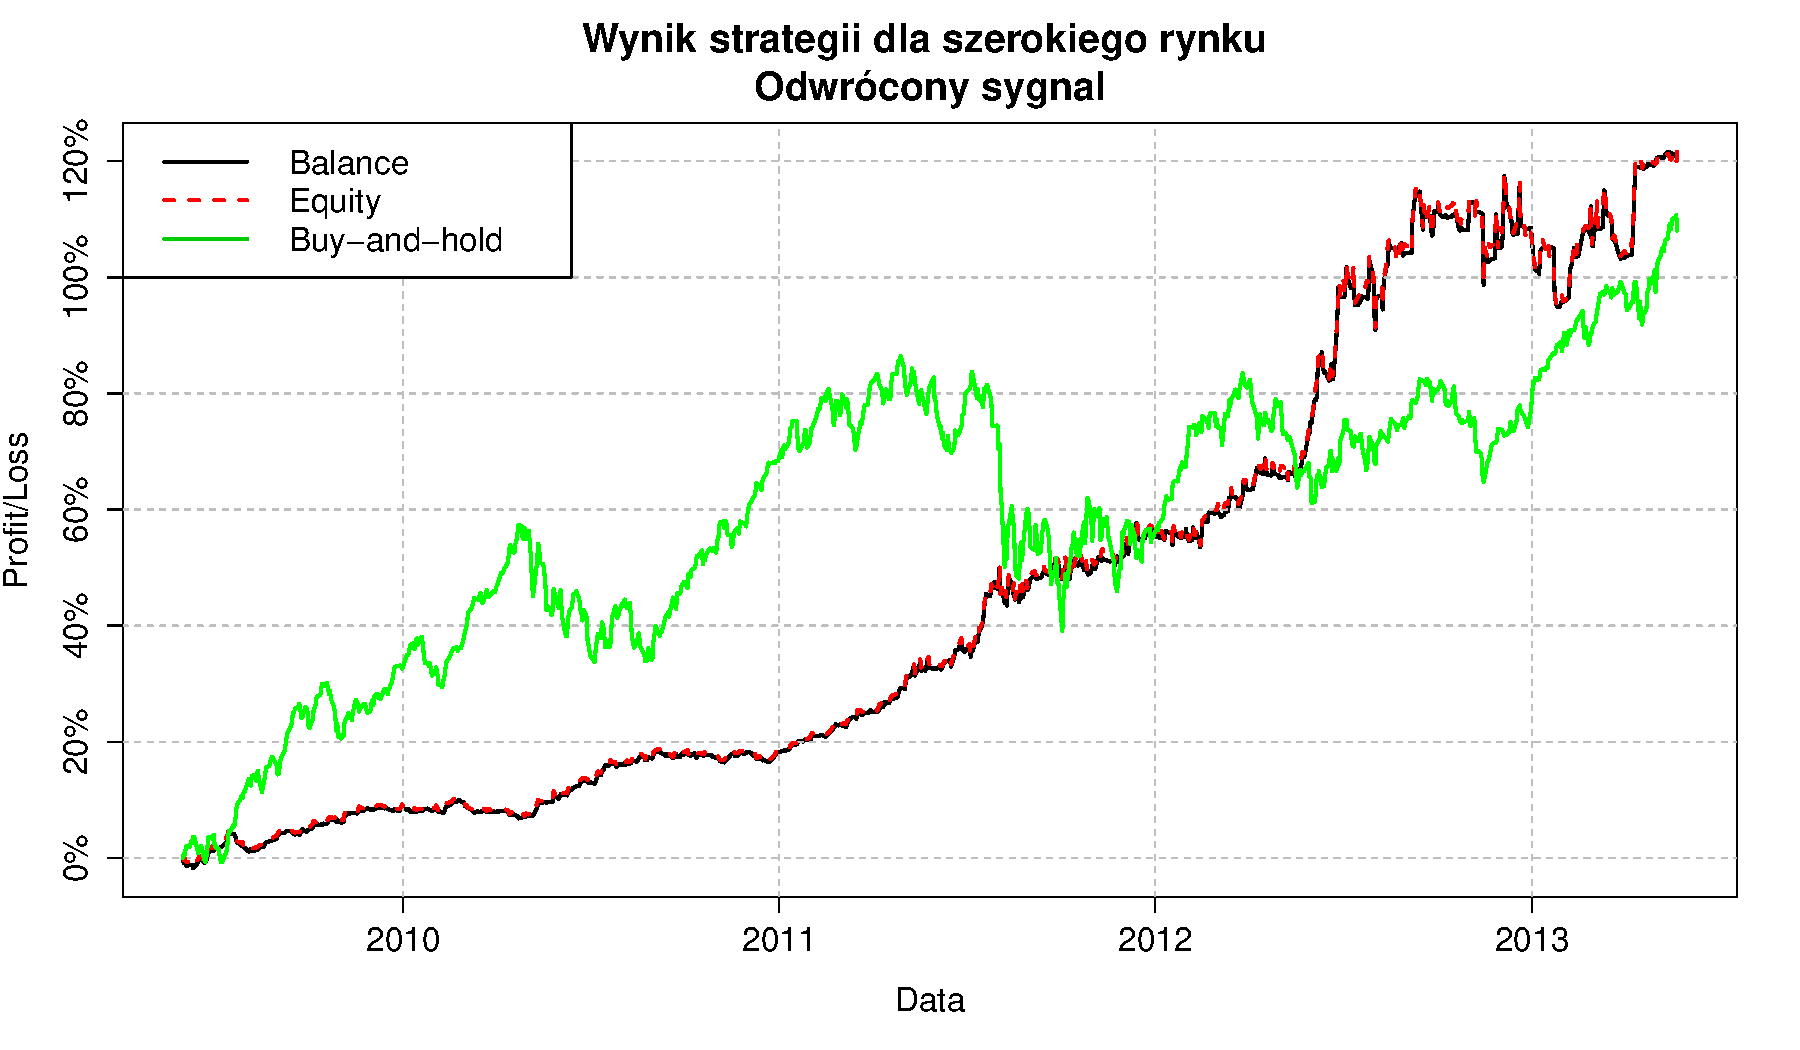
\includegraphics[width=110mm,height = 55mm]{revallmarket}
\vspace{-10pt}
\caption{Krzywe Balance i Equity dla odwróconej strategii RegTrend zastosowanej dla szerokiego rynku, porównane ze strategią ,,Buy-and-hold''.}\vspace{-10pt}
\caption*{Źródło: Obliczenia własne - R Project}\vspace{-20pt}
\label{fig:revallmarket}
\end{figure}

Powyższy wykres (rys. \ref{fig:revallmarket}) wskazuje , że pierwotne założenia odnośnie kontynuacji trendu w analizowanym okresie nie sprawdziły się, jednak sygnał odwrotny dał zadowalający rezultat, od pewnego momentu przewyższający strategię porównawczą. W analizowanym okresie zysk ze strategii wyniósłby 122\% (22\% średniorocznie)w porównaniu do 108\% (20.1\% średniorocznie) dla ,,Buy-and-hold''.

Należy jednak zwrócić uwagę, iż w przypadku analizy wyniku backtestu znaczenie ma kształt krzywych Balance i Equity. Może zdarzyć się sytuacja, w której główny zysk pochodzi z pojedynczej transakcji lub z jednego określonego okresu. W przypadku odwróconego RegTrend krzywe Equity i Balance są dosyć gładkie w początkowym okresie, jednak w ostatnim roku zmienność zwrotów drastycznie rośnie (rys. \ref{fig:volchange}).
\begin{figure}[H]
\centering
\vspace{-10pt}
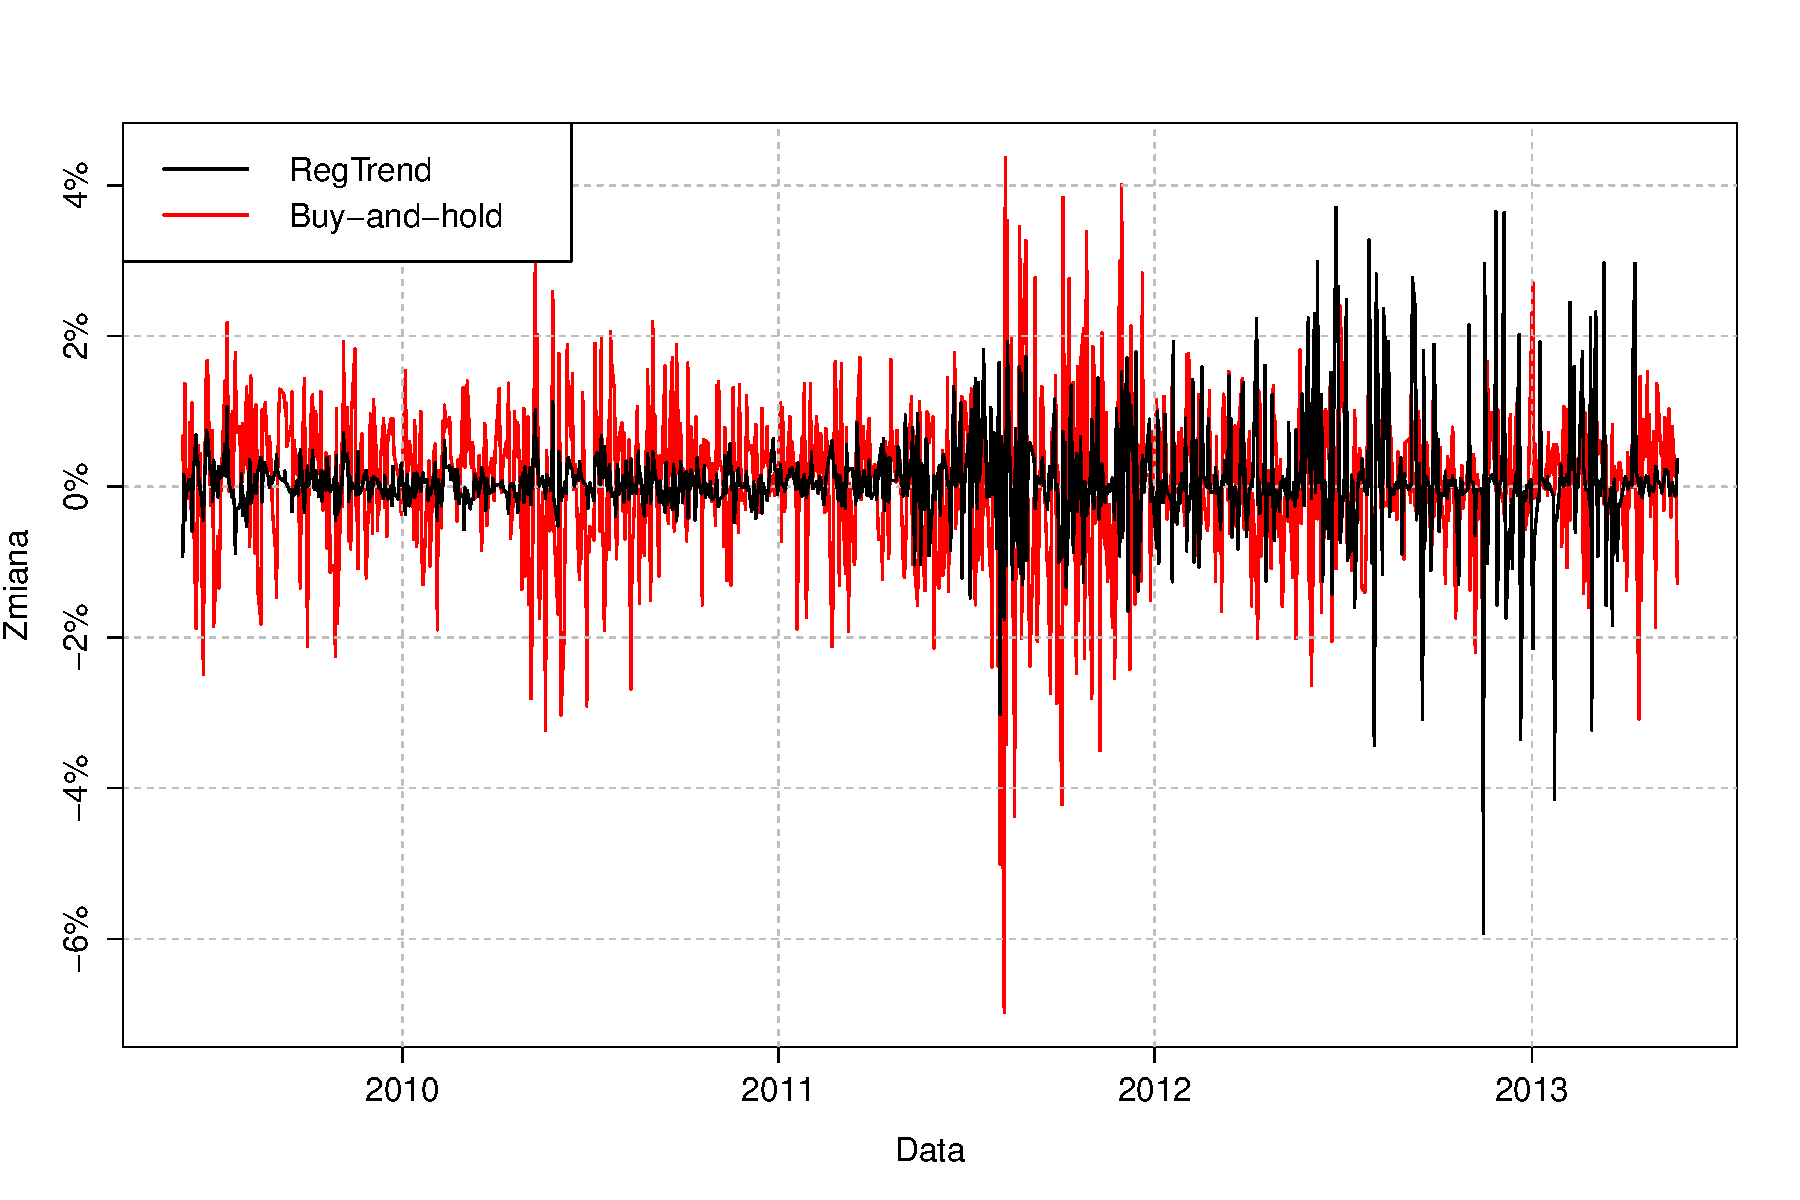
\includegraphics[width=100mm,height = 55mm]{volchange}
\vspace{-10pt}
\caption{Krzywe logarytmicznych zmian Balance dla odwróconej wersji RegTrend i strategii "Buy-and-hold".}\vspace{-10pt}
\caption*{Źródło: Obliczenia własne - R Project}
\label{fig:volchange}\vspace{-10pt}
\end{figure}


Dalsza analiza strategii powinna ująć wrażliwość na zmianę kosztów transakcyjnych. W wielu przypadkach są one w stanie diametralnie zmienić wynik, w szczególności jeżeli strategia wykonuje bardzo dużo transakcji. % Powyższe wyniki prezentowane były z założeniem, iż prowizja wynosi 0.02\% wartości transakcji.

Poniżej (rys.\ref{fig:commission}) prezentowane są krzywe Balance w zależności od kilku wybranych wielkości prowizji:
\begin{figure}[H]
\centering
\vspace{-10pt}
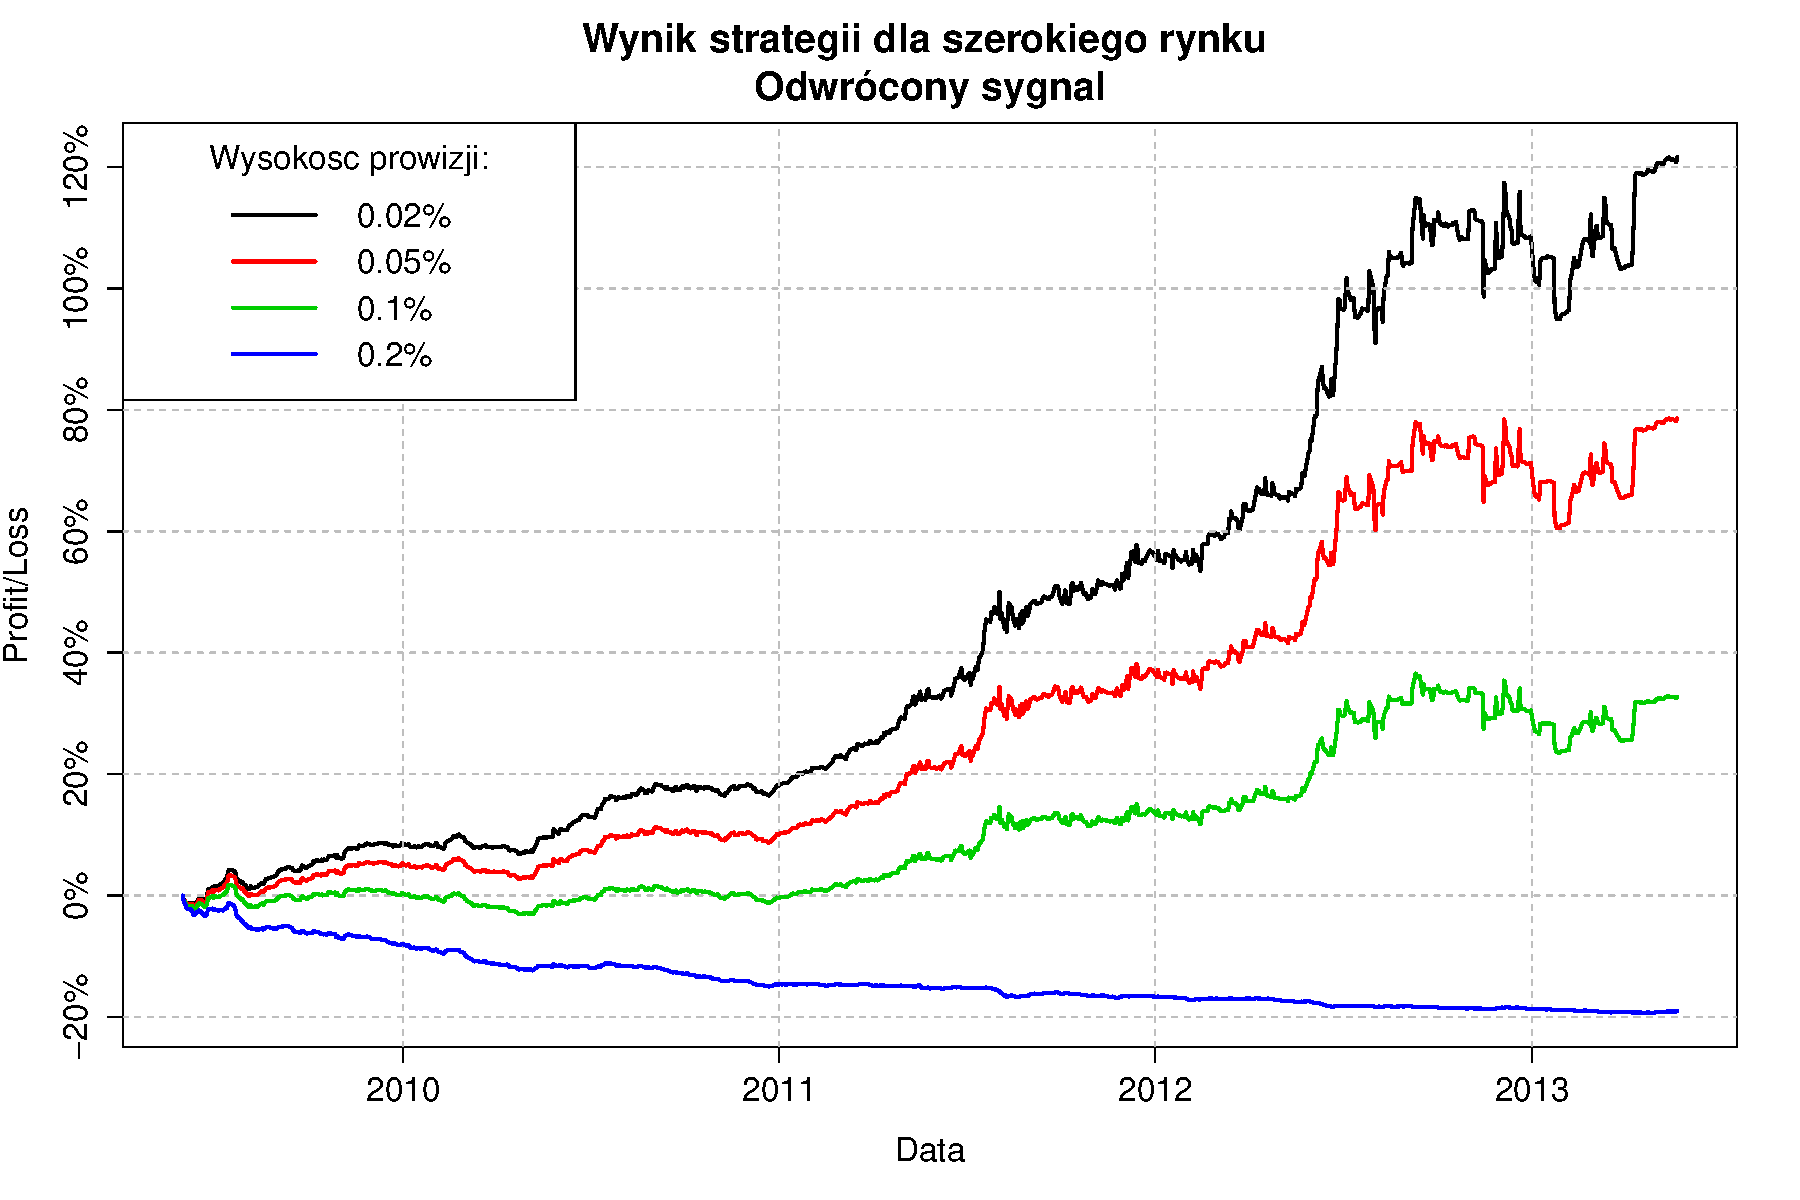
\includegraphics[width=120mm,height = 70mm]{commission}
\vspace{-10pt}
\caption{Krzywe Balance w przypadku różnych wysokości prowizji.}
\caption*{Źródło: Obliczenia własne - R Project}
\label{fig:commission}
\end{figure}

Na korzyść strategii przemawia fakt, że nawet pięciokrotne podwyższenie kosztów transakcyjnych nie spowodowało, że strategia zaczęła diametralnie tracić.

\section{Wnioski}

Pierwotnie przyjęte założenia strategii, mówiące że jeżeli występuje dodatnie nachylenie krzywej regresji czasu względem ceny wyznaczonej dla ostatnich dwóch miesięcy, wtedy dany aktyw znajduje się w trendzie wzrostowym, który będzie kontynuowany - należy więc zająć pozycję długą (analogicznie dla ujemnego nachylenia krzywej regresji), okazały się w przypadku rynku NASDAQ nieadekwatne, jednak ich przeciwieństwo dało zadowalające wyniki. 

Fakt, iż wyniki odwróconej strategii były zbliżone do rynkowych sugeruje, że reguła decyzyjna polegająca na monitorowaniu współczynnika nachylenia regresji może być użyteczna w handlu algorytmicznym. Dodatkowo podejście oparte na strumieniach danych i oknach, pozwala na monitorowanie bardzo dużej ilości aktywów, co może szczególne znaczenie w kontekście redukcji ryzyka poprzez dywersyfikację portfela.

\chapter{Wnioski końcowe}

W pracy zaprezentowano podejście do monitorowania strumieni danych przy pomocy  algorytmów prostej regresji: metody najmniejszych kwadratów, największej głębi regresyjnej oraz regresji k najbliższych sąsiadów. Pierwsza metoda wykazała najlepsze własności w przypadku braku występowania obserwacji odstających, jednak jej wskazania znaczenie się pogorszyły wraz pojawienia się nietypowych obserwacji. W tej sytuacji zdecydowanie lepszym algorytmem okazała się metoda największej głębi regresyjnej.

Stosując wyżej wymieniony metody należy mieć na uwadze między innymi fakt, iż dla strumienia o częstych zmianach reżimu cecha odporności określonej procedury statystycznej może być niepożądana, co zostało pokazane w symulacjach. W takim przypadku lepsze efekty można uzyskać poprzez skrócenie okna na którym wyznaczany jest model.

Na szczególną uwagę zasługuje techniczny aspekt analizy wielkich zbiorów danych jakim jest dostępność wygodnych narzędzi ułatwiających prowadzenie obliczeń równoległych. Przykładowo w pakiecie R, by móc skorzystać z większej ilości rdzeni procesora wystarczy zaledwie kilka linijek dodatkowego kodu. Jednocześnie najbardziej wydajne techniki związane z obliczeniami nadal wymagają dużej wiedzy i zasobów finansowych.

\newpage


\listoffigures	

\newpage
\listoftables

\newpage

%\bibliographystyle{plain}
%\DeclareNameAlias{sortname}{first-last}
\bibliographystyle{plain}
\renewcommand\bibname{Literatura}
\bibliography{bibliografia}


\end{document}